% =====================================================================
%  SUPPLEMENTARY MATERIAL — companion to:
%    "Bagging-Enhanced Medoid-Based Clustering on Kendall's
%     Two-Dimensional Shape Space"
% =====================================================================
\documentclass[11pt,a4paper]{article}

\usepackage[a4paper,margin=2.4cm]{geometry}
\usepackage{amsmath,amssymb,amsthm}
\usepackage{algorithm}
\usepackage[noend]{algpseudocode}
\usepackage{booktabs}
\usepackage{graphicx}
\usepackage{subcaption}
\usepackage{multirow}
\usepackage{makecell}
\usepackage{xcolor}
\usepackage{microtype}
\usepackage{enumitem}
\usepackage{bm}
\usepackage{tikz}
\usetikzlibrary{arrows.meta,positioning,shapes.geometric,calc,fit,backgrounds,decorations.pathreplacing}
\usepackage{natbib}
\bibliographystyle{plainnat}

\usepackage{hyperref}
\hypersetup{colorlinks=true,linkcolor=blue!55!black,citecolor=blue!55!black,
            urlcolor=blue!55!black,pdfborder={0 0 0}}
\usepackage{cleveref}

\newcommand{\R}{\mathbb{R}}
\newcommand{\C}{\mathbb{C}}
\newcommand{\CP}{\mathbb{C}P}
\newcommand{\Herm}[1]{{#1}^{*}}
\newcommand{\norm}[1]{\|{#1}\|}
\newcommand{\preshape}{S^{2k-3}_{\C}}
\newcommand{\bz}{\mathbf{z}}
\newcommand{\bA}{\mathbf{A}}
\newcommand{\bX}{\mathbf{X}}
\newcommand{\bH}{\mathbf{H}}
\newcommand{\bI}{\mathbf{I}}
\newcommand{\bone}{\mathbf{1}}
\newcommand{\bigOh}{\mathcal{O}}
\newcommand{\ShapeClust}{\texttt{ShapeClust}}
\newcommand{\rmVEG}{\mathrm{VEG}}
\newcommand{\rmVIG}{\mathrm{VIG}}

% Re-prefix tables and figures with "S" so as not to clash with the main paper
\renewcommand{\thetable}{S\arabic{table}}
\renewcommand{\thefigure}{S\arabic{figure}}
\renewcommand{\thealgorithm}{S\arabic{algorithm}}
\renewcommand{\theequation}{S.\arabic{equation}}
\renewcommand{\thesection}{S.\arabic{section}}

\title{Supplementary Material to\\
       ``Bagged Medoid-Based Clustering on Kendall's\\
       Two-Dimensional Shape Space''}
\author{Raydonal Ospina \and
        In\'{a}cio Robson Alves do Nascimento \and
        Get\'{u}lio Jos\'{e} Amorim do Amaral\\[0.3em]
        \small Department of Statistics, Universidade Federal de Pernambuco}
\date{}

\begin{document}
\maketitle

\section*{Contents}

This document supports the main paper. Sections are numbered S.1--S.8 and its
tables, figures and equations are prefixed with an S, so that they never clash
with those of the main paper. Every number reported here was produced by the
\texttt{ShapeClust} package from the scripts distributed with it.

\begin{description}[leftmargin=2.1cm, style=nextline]

\item[Section S.1] \textbf{Scalability tables.} Wall-clock times of the three
  main routines over a grid of sample sizes and landmark counts
  (Table~\ref{tab:scal-nk}), and of the bagging loop as a function of the number
  of bootstrap replicates (Table~\ref{tab:scal-B}). Supports Section~4 of the
  main paper.

\item[Section S.2] \textbf{Complex Bingham simulator and simulation regimes.}
  Full distributional specification, pseudocode for the two exact samplers, the
  group reference directions, and the covariance structures of the isotropic and
  anisotropic regimes. Supports Section~5.2 of the main paper.

\item[Section S.3] \textbf{Simulated objects, group alignment, and real-data
  configurations.} The three template shapes; the effect of the group rotation on
  a Complex Bingham pre-shape, shown in landmark space; the between- and
  within-group Riemannian variances of every simulated scenario
  (Table~\ref{tab:sim-var}); the sand-grain outlines by provenance; and the mean
  orang-utan cranial configuration by sex.

\item[Section S.4] \textbf{Full simulation tables.} All twenty-four scenarios:
  medians, standard deviations and paired Wilcoxon $p$-values for both base
  clusterers and both validation indices (Tables~\ref{tab:pam-bing-k4}
  to~\ref{tab:rkm-aniso-k34}). Supports Table~1 of the main paper.

\item[Section S.5] \textbf{Split-violin visualizations.} The complete set of
  forty-eight panels, one for every (regime, algorithm, index, landmark count,
  sample size) combination. Supports Figure~3 of the main paper.

\item[Section S.6] \textbf{Wall-clock time tables.} Running times of both base
  clusterers, with and without bagging, in every regime.

\item[Section S.7] \textbf{Real-world biplots and timing.} Principal-component
  biplots of the two real datasets and the corresponding running times.

\item[Section S.8] \textbf{Sensitivity to the choice of shape-space distance.}
  The study re-run with the full Procrustes distance $d_F$ in place of the
  Riemannian distance $\rho$, and whether the conclusions survive the
  substitution (Table~\ref{tab:dF-vs-rho}).

\end{description}

\clearpage

\section{Scalability tables}
\label{sec:scal}

\begin{table}[h]
\centering
\caption{Median wall-clock time (seconds) over three replications for the
  three main routines of \texttt{ShapeClust} on a factorial grid of sample
  size $n$ and landmark count $k$ ($K=3$, $m=5$). Values below $1$ ms are
  reported as $0.000$. Referenced from Section~4 of the main paper.}
\label{tab:scal-nk}
\small
\begin{tabular}{cc rrr}
\toprule
$n$ & $k$ & Distance matrix & Shape-PAM & Shape-rankkmed \\
\midrule
  50 &  4 & $0.000$ & $0.007$ & $0.005$ \\
 100 &  4 & $0.000$ & $0.018$ & $0.007$ \\
 200 &  4 & $0.001$ & $0.055$ & $0.017$ \\
 500 &  4 & $0.009$ & $0.175$ & $0.084$ \\
1000 &  4 & $0.037$ & $0.470$ & $0.283$ \\
\midrule
  50 & 24 & $0.000$ & $0.008$ & $0.004$ \\
 100 & 24 & $0.001$ & $0.014$ & $0.007$ \\
 200 & 24 & $0.002$ & $0.042$ & $0.017$ \\
 500 & 24 & $0.011$ & $0.137$ & $0.071$ \\
1000 & 24 & $0.049$ & $0.422$ & $0.281$ \\
\midrule
  50 & 50 & $0.000$ & $0.007$ & $0.004$ \\
 100 & 50 & $0.001$ & $0.018$ & $0.008$ \\
 200 & 50 & $0.002$ & $0.052$ & $0.017$ \\
 500 & 50 & $0.015$ & $0.151$ & $0.095$ \\
1000 & 50 & $0.069$ & $0.432$ & $0.336$ \\
\bottomrule
\end{tabular}
\end{table}

\begin{table}[h]
\centering
\caption{Wall-clock time of BagClust1 (Shape-PAM base, $n=200$, $k=24$,
  $K=3$) as a function of the number of bootstrap replicates $B$.
  Referenced from Section~4 of the main paper.}
\label{tab:scal-B}
\small
\begin{tabular}{rrr}
\toprule
$B$ & Time (s) & Time per replicate (s) \\
\midrule
 10 & $0.54$ & $0.054$ \\
 25 & $1.11$ & $0.044$ \\
 50 & $2.03$ & $0.041$ \\
100 & $4.06$ & $0.041$ \\
\bottomrule
\end{tabular}
\end{table}

All timings were obtained with \texttt{ShapeClust} 0.2.0 (C\raisebox{0.3ex}{\scriptsize++}
core via \texttt{Rcpp} and \texttt{RcppArmadillo}) on a single core of an
Intel Core i7-1165G7 CPU, R 4.3.3. The per-replicate cost in the second
table stabilizes at about $41$ ms, confirming that the overhead of the
bootstrap loop and of the Hungarian label alignment is negligible relative
to the base clusterer.

\clearpage

\section{Complex Bingham simulator and simulation regimes}
\label{sec:bingham-sim}
% =====================================================================

The Complex Bingham distribution on the pre-shape sphere $\preshape$ has
the density
\begin{equation}
  \label{eq:cbingham-density}
  f(\bz \mid \bA)
  = c(\bA)^{-1}\exp\!\bigl(\Herm{\bz}\bA\bz\bigr),
\end{equation}
with $\bA$ Hermitian, ordered eigenvalues
$\lambda_1<\lambda_2<\cdots<\lambda_k=0$, and normalising constant
\[
  c(\bA)
  = 2\pi^{k}\sum_{i=1}^{k}\left[\prod_{j\ne i}(\lambda_i-\lambda_j)\right]^{-1}
                                       \exp(\lambda_i).
\]
The Simplex-truncation generator of \citet{kent2004simulation} produces
draws by writing $k-1$ truncated-exponential variables in polar
coordinates. Algorithm~\ref{alg:exp-sim} produces the truncated
exponentials; Algorithm~\ref{alg:bin-sim} produces the Complex Bingham
draw.

\begin{algorithm}[t]
\caption{Truncated-exponential generator
  \citep{kent2004simulation}.}
\label{alg:exp-sim}
\begin{algorithmic}[1]
\Require Concentration parameters $\lambda_1,\ldots,\lambda_k$.
\Ensure  A vector $\bm{S}$ from the truncated exponential distribution.
\State Simulate $U_j\sim\mathcal{U}[0,1]$, $j=1,\ldots,k$.
\State Compute $S'_j = -(1/\lambda_j)\log\bigl(1-U_j(1-e^{-\lambda_j})\bigr)$
       for $j=1,\ldots,k$.
\If{$\sum_{j=1}^{k} S'_j < 1$}
  \State Set $\bm{S} \gets (S'_1,\ldots,S'_k)^\top$.
\Else
  \State Reject and return to step~1.
\EndIf
\State \Return $\bm{S}$.
\end{algorithmic}
\end{algorithm}

\begin{algorithm}[t]
\caption{Complex Bingham generator
  \citep{kent2004simulation}.}
\label{alg:bin-sim}
\begin{algorithmic}[1]
\Require Concentration parameters $\lambda_1,\ldots,\lambda_k$.
\Ensure  A vector $\bz=(z_1,\ldots,z_k)^\top$ from the Complex Bingham
         distribution.
\State Run Algorithm~\ref{alg:exp-sim} to obtain $\bm{S}=(S_1,\ldots,S_k)^\top$
       with $S_j\sim\text{Texp}(\lambda_j)$.
\If{$\sum_{j=1}^{k-1} S_j < 1$}
  \State Set $S_k \gets 1-\sum_{j=1}^{k-1} S_j$.
\Else
  \State Return to step~1.
\EndIf
\State Generate independent angles $\theta_j\sim\mathcal{U}[0,2\pi)$,
       $j=1,\ldots,k$.
\State Compute $z_j = S_j^{1/2}\exp(\mathrm{i}\,\theta_j)$, $j=1,\ldots,k$.
\State \Return $\bz=(z_1,\ldots,z_k)^\top$.
\end{algorithmic}
\end{algorithm}

\paragraph{Rotation vectors used in the simulation.} To create three
distinct groups in the Bingham regime, the technique of complex-vector
rotation of \citet{amaral2007pivotal} is applied: an original vector
$\mathbf{v}_0$ is rotated towards a group-specific reference vector
$\mathbf{v}_g$, $g=1,2,3$, leaving the orthogonal complement of the plane
they span unchanged. For $k=4$ landmarks we use
$\mathbf{v}_{1}=(0,0,1,1)$, $\mathbf{v}_{2}=(1,1,0,0)$ and
$\mathbf{v}_{3}=(0,1,1,0)$. For $k=24$ landmarks we use the
twelve-block vectors
$\mathbf{v}_{1,k=24}=(0^{12},1^{12})$,
$\mathbf{v}_{2,k=24}=(1^{12},0^{12})$,
$\mathbf{v}_{3,k=24}=(0^{6},1^{12},0^{6})$,
where $a^{m}$ denotes $m$ copies of the scalar $a$. The rotation vectors
are unrelated to the $\{\lambda_j\}$, which control only concentration.

\paragraph{Isotropic and anisotropic landmark covariances.} In the
landmark regimes the three groups have predefined mean configurations of
a square, a rectangle, and a trapezoid; their explicit coordinates for
$k=4$ are given in Table~\ref{tab:mean-configs}.

\begin{table}[t]
\centering
\caption{Mean configurations of the three landmark groups for $k=4$:
  (a) square, (b) rectangle, (c) trapezoid.}
\label{tab:mean-configs}
\small
\begin{tabular}{cc cc cc cc}
\toprule
& \multicolumn{2}{c}{(a) Square}
& \multicolumn{2}{c}{(b) Rectangle}
& \multicolumn{2}{c}{(c) Trapezoid} \\
\cmidrule(lr){2-3}\cmidrule(lr){4-5}\cmidrule(lr){6-7}
$\ell$ & $x$ & $y$ & $x$ & $y$ & $x$ & $y$ \\
\midrule
1 & 0  & 0  & 0  & 0  & 0  & 0  \\
2 & 0  & 10 & 10 & 0  & 40 & 0  \\
3 & 10 & 10 & 0  & 20 & 0  & 30 \\
4 & 10 & 0  & 10 & 20 & 20 & 30 \\
\bottomrule
\end{tabular}
\end{table}

For $k=34$ the mean configurations of the square, rectangle, and
trapezoid are obtained by adding $30$ intermediate landmarks evenly
spaced along the perimeter of each polygon. Landmarks are perturbed by
a multivariate Gaussian with group-specific covariance $\Sigma_i$,
$i=1,2,3$. Under isotropy, $\Sigma_i=\sigma_i^2 \bI_{mk\times mk}$; under
anisotropy, following \citet{preston2010two},
\begin{equation}
  \label{eq:aniso}
  \Sigma_i = \sigma_i^2\,\bigl[\bone_{k}\bone_{k}^\top
   + (\gamma-1)\bI_{k\times k}\bigr] \otimes
   \bigl[\bone_{m}\bone_{m}^\top + (\gamma-1)\bI_{m\times m}\bigr]
   / \gamma^2,
\end{equation}
with anisotropy parameter $\gamma=4$. Object orientation is randomized
by a rotation around the $y$-axis through an angle drawn from a von
Mises distribution (\texttt{rvm} of the \texttt{CircStats} R package),
as in \citet{vinue2016means}.


% =====================================================================
\section{Simulated objects, group alignment, and real-data configurations}
\label{sec:objects}

This section collects the descriptive figures of the study design: the three
template objects used by the landmark regimes, the effect of the group rotation
on a Complex Bingham pre-shape, the raw outlines of the two real datasets, and
the between/within variability of the simulated pre-shape data.

\subsection*{Template objects}

\begin{figure}[h]
\centering
\begin{subfigure}{0.31\textwidth}\centering
  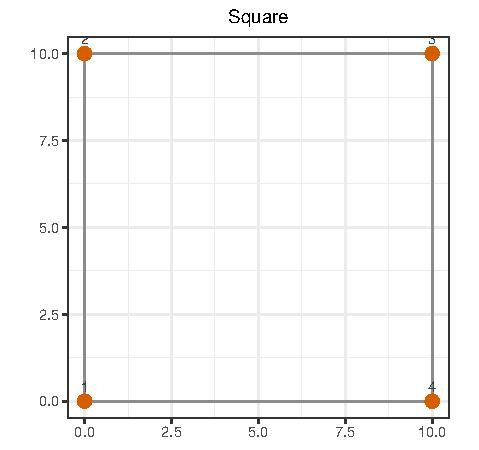
\includegraphics[width=\linewidth]{figures/template_square.pdf}
  \caption{Square}
\end{subfigure}\hfill
\begin{subfigure}{0.31\textwidth}\centering
  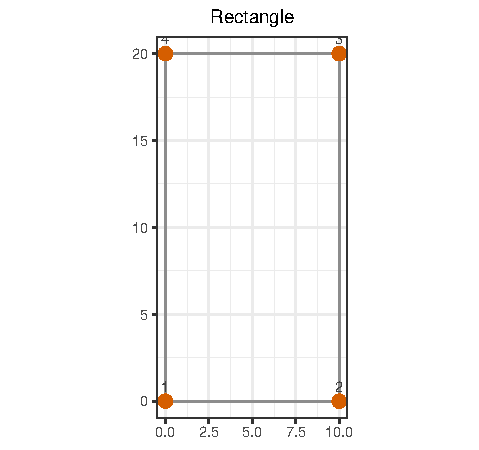
\includegraphics[width=\linewidth]{figures/template_rectangle.pdf}
  \caption{Rectangle}
\end{subfigure}\hfill
\begin{subfigure}{0.31\textwidth}\centering
  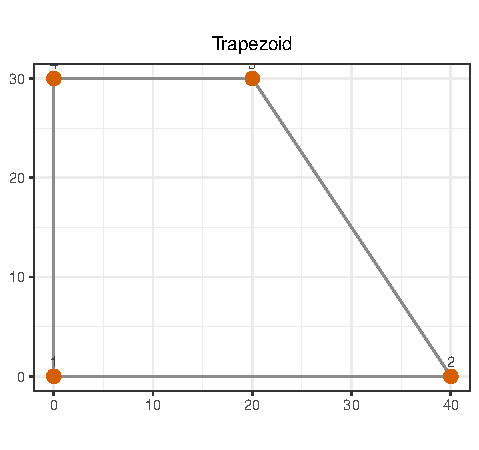
\includegraphics[width=\linewidth]{figures/template_trapezoid.pdf}
  \caption{Trapezoid}
\end{subfigure}
\caption{The three predefined mean configurations of the isotropic and
  anisotropic regimes, shown for $k=4$ landmarks (numbered). For $k=34$ the same
  three outlines are densified by interpolating additional landmarks along the
  perimeter, so the group means remain a square, a rectangle, and a trapezoid.}
\label{fig:templates}
\end{figure}

\subsection*{Effect of the group rotation on a pre-shape}

In the Complex Bingham regime the three groups are produced from a single
distribution by rotating its concentration pole onto three different reference
directions. Figure~\ref{fig:preshape-align} shows what that operation does in
landmark space: the same simulated object is mapped back through the inverse
Helmert projection before and after each rotation. The rotation is an isometry
of the pre-shape sphere, so the concentration is preserved and only the modal
shape changes, which is precisely what creates three groups that differ in shape
but not in dispersion.

\begin{figure}[h]
\centering
\begin{subfigure}{0.24\textwidth}\centering
  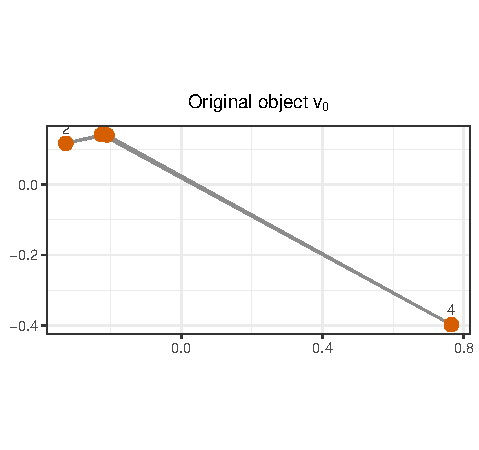
\includegraphics[width=\linewidth]{figures/preshape_g0_k4_c1.pdf}
  \caption{Original object}
\end{subfigure}\hfill
\begin{subfigure}{0.24\textwidth}\centering
  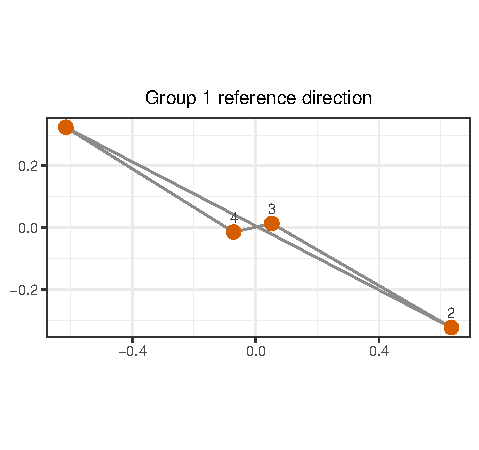
\includegraphics[width=\linewidth]{figures/preshape_g1_k4_c1.pdf}
  \caption{Rotated to group 1}
\end{subfigure}\hfill
\begin{subfigure}{0.24\textwidth}\centering
  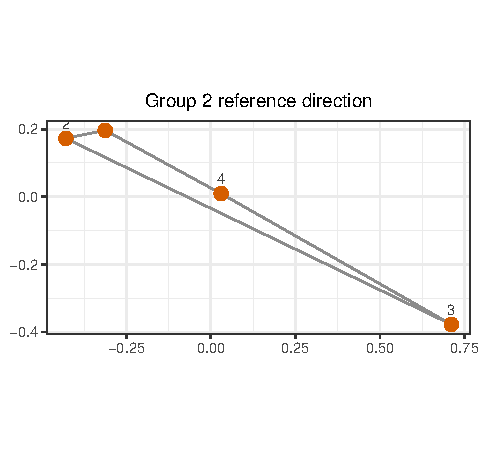
\includegraphics[width=\linewidth]{figures/preshape_g2_k4_c1.pdf}
  \caption{Rotated to group 2}
\end{subfigure}\hfill
\begin{subfigure}{0.24\textwidth}\centering
  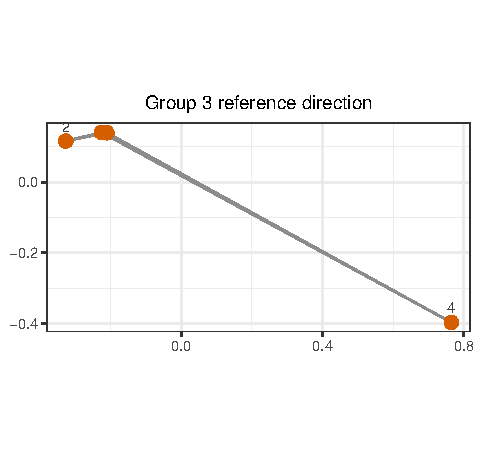
\includegraphics[width=\linewidth]{figures/preshape_g3_k4_c1.pdf}
  \caption{Rotated to group 3}
\end{subfigure}
\caption{Landmark positions of one Complex Bingham pre-shape ($k=4$,
  well-separated setting) before and after alignment to each of the three group
  reference directions.}
\label{fig:preshape-align}
\end{figure}

\subsection*{Variability of the simulated pre-shape datasets}

Table~\ref{tab:sim-var} reports the Riemannian between-group variance (VEG), the
within-group variance (VIG), and their ratio, averaged over $20$ simulated
datasets per scenario. The ratio behaves as the design intends: it is very large
in the well-separated setting and falls by one to two orders of magnitude in the
overlapping one. It also falls with the landmark count at a fixed concentration,
from about $5$ at $k=4$ to about $1.6$ at $k=24$ in the overlapping setting.
This is the quantitative counterpart of the statement in the main paper that a
larger landmark count makes the task harder, and it is why the concentration of
the overlapping scenario has to be raised from $\lambda=9$ to $\lambda=30$ when
$k$ goes from $4$ to $24$.

\begin{table}[h]
\centering
\caption{Between-group (VEG) and within-group (VIG) Riemannian variances of the
  simulated pre-shape datasets, averaged over $20$ replications per scenario.
  Overlap~1 is the well-separated setting, Overlap~2 the overlapping one.}
\label{tab:sim-var}
\small
\begin{tabular}{cccrcr}
\toprule
$k$ & $n$ & Overlap & $\lambda$ & VEG\;/\;VIG & Ratio \\
\midrule
 4 &  30 & 1 & $200$ & $2.10\;/\;0.012$ & $174.1$ \\
 4 &  30 & 2 & $9$   & $1.30\;/\;0.300$ & $4.4$ \\
 4 & 150 & 1 & $200$ & $2.08\;/\;0.011$ & $192.4$ \\
 4 & 150 & 2 & $9$   & $1.36\;/\;0.265$ & $5.1$ \\
\midrule
24 &  30 & 1 & $200$ & $2.19\;/\;0.193$ & $11.4$ \\
24 &  30 & 2 & $30$  & $2.07\;/\;1.368$ & $1.5$ \\
24 & 150 & 1 & $200$ & $2.19\;/\;0.175$ & $12.5$ \\
24 & 150 & 2 & $30$  & $2.21\;/\;1.341$ & $1.7$ \\
\bottomrule
\end{tabular}
\end{table}

\subsection*{Real datasets}

\begin{figure}[h]
\centering
\begin{subfigure}{0.42\textwidth}\centering
  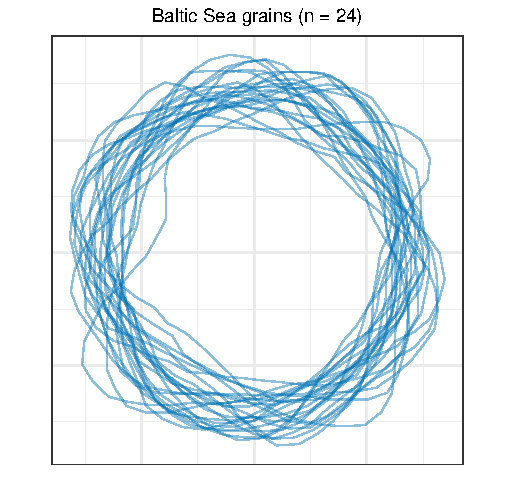
\includegraphics[width=\linewidth]{figures/sand_sea.pdf}
  \caption{Baltic Sea}
\end{subfigure}\hfill
\begin{subfigure}{0.42\textwidth}\centering
  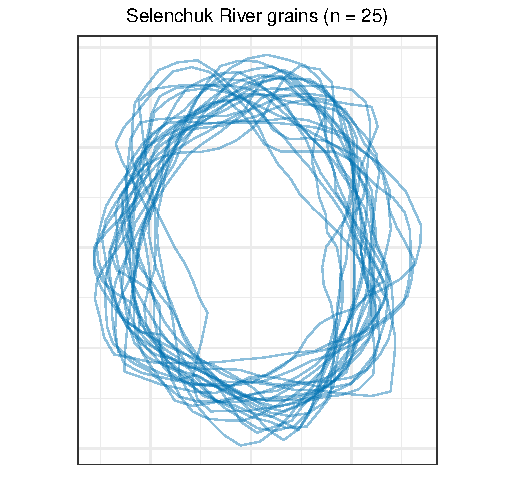
\includegraphics[width=\linewidth]{figures/sand_river.pdf}
  \caption{Selenchuk River}
\end{subfigure}
\caption{Sand-grain outlines by provenance, each described by $50$ landmarks and
  drawn after centering and scaling. The two provenances overlap substantially,
  consistent with the between/within variance ratio of $0.97$ reported in the
  main paper.}
\label{fig:sand-outlines}
\end{figure}

\begin{figure}[h]
\centering
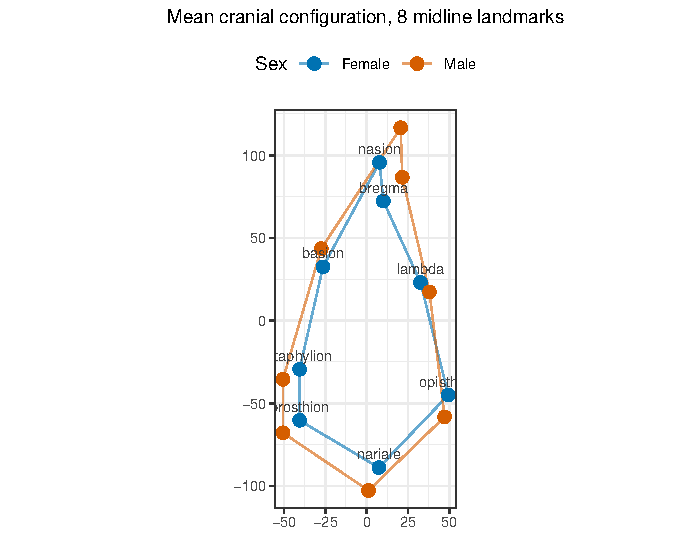
\includegraphics[width=0.62\textwidth]{figures/orang_landmarks.pdf}
\caption{Mean cranial configuration of the orang-utan data by sex, over the eight
  midline landmarks (nariale, prosthion, staphylion, basion, nasion, bregma,
  lambda, opisthion) of \citet{o1989morphometric}. The male mean is larger and
  differently proportioned in the facial block; it is this difference that the
  clustering algorithms must recover without labels.}
\label{fig:orang-landmarks}
\end{figure}

\clearpage

\section{Full simulation tables}
\label{sec:full-sim-tables}

The twelve tables below report every cell of the design: medians
($\tilde x$), standard deviations ($s$), and one-sided paired Wilcoxon
$p$-values over $100$ Monte~Carlo replications, for both validation
indices, both base clusterers, all three regimes and both landmark
counts. Bold $p$-values reject $H_0$ at $\alpha=0.05$. Scenario~1 is the
well-separated setting, Scenario~2 the overlapping one. In the Complex
Bingham regime the concentration of Scenario~2 is $\lambda_j=9$ for $k=4$
and $\lambda_j=30$ for $k=24$; see Section~5.2 of the main paper for the
calibration argument. All numbers were produced by the \texttt{ShapeClust}
package.

\begin{table}[h]
\centering
\caption{Shape-PAM versus its bagged variant, Bingham regime, $k=4$. Medians ($\tilde x$), standard deviations ($s$) and one-sided paired Wilcoxon $p$-values over $100$ Monte Carlo replications.}
\label{tab:pam-bing-k4}
\footnotesize
\begin{tabular}{cc c cc cc}
\toprule
& & & \multicolumn{2}{c}{\textbf{RI}} & \multicolumn{2}{c}{\textbf{FMI}} \\
\cmidrule(lr){4-5}\cmidrule(lr){6-7}
$n$ & Conc. & Approach & $\tilde x$ ($s$) & $p$-val.\ & $\tilde x$ ($s$) & $p$-val.\ \\
\midrule
$30$ & 1 & Std.\ & $1.000\,(0.000)$ & \multirow{2}{*}{$1.000$} & $1.000\,(0.000)$ & \multirow{2}{*}{$1.000$} \\
     &   & $B{=}100$ & $1.000\,(0.000)$ & & $1.000\,(0.000)$ & \\
$30$ & 2 & Std.\ & $0.956\,(0.044)$ & \multirow{2}{*}{$\mathbf{0.004}$} & $0.930\,(0.071)$ & \multirow{2}{*}{$\mathbf{0.004}$} \\
     &   & $B{=}100$ & $0.956\,(0.046)$ & & $0.930\,(0.074)$ & \\
$150$ & 1 & Std.\ & $1.000\,(0.000)$ & \multirow{2}{*}{$1.000$} & $1.000\,(0.000)$ & \multirow{2}{*}{$1.000$} \\
     &   & $B{=}100$ & $1.000\,(0.000)$ & & $1.000\,(0.000)$ & \\
$150$ & 2 & Std.\ & $0.947\,(0.020)$ & \multirow{2}{*}{$\mathbf{0.001}$} & $0.920\,(0.030)$ & \multirow{2}{*}{$\mathbf{0.001}$} \\
     &   & $B{=}100$ & $0.948\,(0.019)$ & & $0.921\,(0.029)$ & \\
\bottomrule
\end{tabular}
\end{table}

\begin{table}[h]
\centering
\caption{Shape-PAM versus its bagged variant, Bingham regime, $k=24$. Medians ($\tilde x$), standard deviations ($s$) and one-sided paired Wilcoxon $p$-values over $100$ Monte Carlo replications.}
\label{tab:pam-bing-k24}
\footnotesize
\begin{tabular}{cc c cc cc}
\toprule
& & & \multicolumn{2}{c}{\textbf{RI}} & \multicolumn{2}{c}{\textbf{FMI}} \\
\cmidrule(lr){4-5}\cmidrule(lr){6-7}
$n$ & Conc. & Approach & $\tilde x$ ($s$) & $p$-val.\ & $\tilde x$ ($s$) & $p$-val.\ \\
\midrule
$30$ & 1 & Std.\ & $1.000\,(0.000)$ & \multirow{2}{*}{$1.000$} & $1.000\,(0.000)$ & \multirow{2}{*}{$1.000$} \\
     &   & $B{=}100$ & $1.000\,(0.000)$ & & $1.000\,(0.000)$ & \\
$30$ & 2 & Std.\ & $0.797\,(0.081)$ & \multirow{2}{*}{$\mathbf{<\!0.001}$} & $0.680\,(0.126)$ & \multirow{2}{*}{$\mathbf{<\!0.001}$} \\
     &   & $B{=}100$ & $0.841\,(0.080)$ & & $0.745\,(0.125)$ & \\
$150$ & 1 & Std.\ & $1.000\,(0.000)$ & \multirow{2}{*}{$1.000$} & $1.000\,(0.000)$ & \multirow{2}{*}{$1.000$} \\
     &   & $B{=}100$ & $1.000\,(0.000)$ & & $1.000\,(0.000)$ & \\
$150$ & 2 & Std.\ & $0.833\,(0.031)$ & \multirow{2}{*}{$\mathbf{<\!0.001}$} & $0.747\,(0.047)$ & \multirow{2}{*}{$\mathbf{<\!0.001}$} \\
     &   & $B{=}100$ & $0.896\,(0.032)$ & & $0.842\,(0.048)$ & \\
\bottomrule
\end{tabular}
\end{table}

\begin{table}[h]
\centering
\caption{Shape-rankkmed versus its bagged variant, Bingham regime, $k=4$. Medians ($\tilde x$), standard deviations ($s$) and one-sided paired Wilcoxon $p$-values over $100$ Monte Carlo replications.}
\label{tab:rkm-bing-k4}
\footnotesize
\begin{tabular}{cc c cc cc}
\toprule
& & & \multicolumn{2}{c}{\textbf{RI}} & \multicolumn{2}{c}{\textbf{FMI}} \\
\cmidrule(lr){4-5}\cmidrule(lr){6-7}
$n$ & Conc. & Approach & $\tilde x$ ($s$) & $p$-val.\ & $\tilde x$ ($s$) & $p$-val.\ \\
\midrule
$30$ & 1 & Std.\ & $1.000\,(0.051)$ & \multirow{2}{*}{$\mathbf{0.029}$} & $1.000\,(0.078)$ & \multirow{2}{*}{$\mathbf{0.030}$} \\
     &   & $B{=}100$ & $1.000\,(0.000)$ & & $1.000\,(0.000)$ & \\
$30$ & 2 & Std.\ & $0.716\,(0.111)$ & \multirow{2}{*}{$\mathbf{<\!0.001}$} & $0.566\,(0.169)$ & \multirow{2}{*}{$\mathbf{<\!0.001}$} \\
     &   & $B{=}100$ & $0.828\,(0.108)$ & & $0.727\,(0.164)$ & \\
$150$ & 1 & Std.\ & $1.000\,(0.057)$ & \multirow{2}{*}{$0.091$} & $1.000\,(0.081)$ & \multirow{2}{*}{$0.091$} \\
     &   & $B{=}100$ & $1.000\,(0.000)$ & & $1.000\,(0.000)$ & \\
$150$ & 2 & Std.\ & $0.680\,(0.056)$ & \multirow{2}{*}{$\mathbf{<\!0.001}$} & $0.528\,(0.080)$ & \multirow{2}{*}{$\mathbf{<\!0.001}$} \\
     &   & $B{=}100$ & $0.873\,(0.086)$ & & $0.808\,(0.120)$ & \\
\bottomrule
\end{tabular}
\end{table}

\begin{table}[h]
\centering
\caption{Shape-rankkmed versus its bagged variant, Bingham regime, $k=24$. Medians ($\tilde x$), standard deviations ($s$) and one-sided paired Wilcoxon $p$-values over $100$ Monte Carlo replications.}
\label{tab:rkm-bing-k24}
\footnotesize
\begin{tabular}{cc c cc cc}
\toprule
& & & \multicolumn{2}{c}{\textbf{RI}} & \multicolumn{2}{c}{\textbf{FMI}} \\
\cmidrule(lr){4-5}\cmidrule(lr){6-7}
$n$ & Conc. & Approach & $\tilde x$ ($s$) & $p$-val.\ & $\tilde x$ ($s$) & $p$-val.\ \\
\midrule
$30$ & 1 & Std.\ & $1.000\,(0.057)$ & \multirow{2}{*}{$0.050$} & $1.000\,(0.088)$ & \multirow{2}{*}{$0.050$} \\
     &   & $B{=}100$ & $1.000\,(0.000)$ & & $1.000\,(0.000)$ & \\
$30$ & 2 & Std.\ & $0.629\,(0.056)$ & \multirow{2}{*}{$\mathbf{<\!0.001}$} & $0.422\,(0.087)$ & \multirow{2}{*}{$\mathbf{<\!0.001}$} \\
     &   & $B{=}100$ & $0.676\,(0.083)$ & & $0.498\,(0.128)$ & \\
$150$ & 1 & Std.\ & $1.000\,(0.035)$ & \multirow{2}{*}{$0.211$} & $1.000\,(0.050)$ & \multirow{2}{*}{$0.211$} \\
     &   & $B{=}100$ & $1.000\,(0.014)$ & & $1.000\,(0.021)$ & \\
$150$ & 2 & Std.\ & $0.632\,(0.042)$ & \multirow{2}{*}{$\mathbf{<\!0.001}$} & $0.449\,(0.062)$ & \multirow{2}{*}{$\mathbf{<\!0.001}$} \\
     &   & $B{=}100$ & $0.812\,(0.079)$ & & $0.721\,(0.110)$ & \\
\bottomrule
\end{tabular}
\end{table}

\begin{table}[h]
\centering
\caption{Shape-PAM versus its bagged variant, Isotropic regime, $k=4$. Medians ($\tilde x$), standard deviations ($s$) and one-sided paired Wilcoxon $p$-values over $100$ Monte Carlo replications.}
\label{tab:pam-iso-k4}
\footnotesize
\begin{tabular}{cc c cc cc}
\toprule
& & & \multicolumn{2}{c}{\textbf{RI}} & \multicolumn{2}{c}{\textbf{FMI}} \\
\cmidrule(lr){4-5}\cmidrule(lr){6-7}
$n$ & Scen. & Approach & $\tilde x$ ($s$) & $p$-val.\ & $\tilde x$ ($s$) & $p$-val.\ \\
\midrule
$30$ & 1 & Std.\ & $0.937\,(0.058)$ & \multirow{2}{*}{$0.950$} & $0.899\,(0.084)$ & \multirow{2}{*}{$0.940$} \\
     &   & $B{=}100$ & $0.917\,(0.061)$ & & $0.869\,(0.089)$ & \\
$30$ & 2 & Std.\ & $0.644\,(0.053)$ & \multirow{2}{*}{$\mathbf{0.020}$} & $0.477\,(0.073)$ & \multirow{2}{*}{$\mathbf{0.025}$} \\
     &   & $B{=}100$ & $0.657\,(0.048)$ & & $0.493\,(0.070)$ & \\
$150$ & 1 & Std.\ & $0.941\,(0.026)$ & \multirow{2}{*}{$\mathbf{0.032}$} & $0.911\,(0.039)$ & \multirow{2}{*}{$\mathbf{0.031}$} \\
     &   & $B{=}100$ & $0.941\,(0.023)$ & & $0.911\,(0.034)$ & \\
$150$ & 2 & Std.\ & $0.643\,(0.027)$ & \multirow{2}{*}{$\mathbf{<\!0.001}$} & $0.502\,(0.039)$ & \multirow{2}{*}{$\mathbf{<\!0.001}$} \\
     &   & $B{=}100$ & $0.649\,(0.024)$ & & $0.519\,(0.033)$ & \\
\bottomrule
\end{tabular}
\end{table}

\begin{table}[h]
\centering
\caption{Shape-PAM versus its bagged variant, Isotropic regime, $k=34$. Medians ($\tilde x$), standard deviations ($s$) and one-sided paired Wilcoxon $p$-values over $100$ Monte Carlo replications.}
\label{tab:pam-iso-k34}
\footnotesize
\begin{tabular}{cc c cc cc}
\toprule
& & & \multicolumn{2}{c}{\textbf{RI}} & \multicolumn{2}{c}{\textbf{FMI}} \\
\cmidrule(lr){4-5}\cmidrule(lr){6-7}
$n$ & Scen. & Approach & $\tilde x$ ($s$) & $p$-val.\ & $\tilde x$ ($s$) & $p$-val.\ \\
\midrule
$30$ & 1 & Std.\ & $1.000\,(0.004)$ & \multirow{2}{*}{$0.500$} & $1.000\,(0.007)$ & \multirow{2}{*}{$0.500$} \\
     &   & $B{=}100$ & $1.000\,(0.000)$ & & $1.000\,(0.000)$ & \\
$30$ & 2 & Std.\ & $0.710\,(0.065)$ & \multirow{2}{*}{$0.688$} & $0.557\,(0.093)$ & \multirow{2}{*}{$0.270$} \\
     &   & $B{=}100$ & $0.699\,(0.067)$ & & $0.557\,(0.088)$ & \\
$150$ & 1 & Std.\ & $1.000\,(0.002)$ & \multirow{2}{*}{$0.074$} & $1.000\,(0.003)$ & \multirow{2}{*}{$0.074$} \\
     &   & $B{=}100$ & $1.000\,(0.001)$ & & $1.000\,(0.002)$ & \\
$150$ & 2 & Std.\ & $0.716\,(0.039)$ & \multirow{2}{*}{$0.993$} & $0.585\,(0.057)$ & \multirow{2}{*}{$0.051$} \\
     &   & $B{=}100$ & $0.702\,(0.046)$ & & $0.591\,(0.050)$ & \\
\bottomrule
\end{tabular}
\end{table}

\begin{table}[h]
\centering
\caption{Shape-rankkmed versus its bagged variant, Isotropic regime, $k=4$. Medians ($\tilde x$), standard deviations ($s$) and one-sided paired Wilcoxon $p$-values over $100$ Monte Carlo replications.}
\label{tab:rkm-iso-k4}
\footnotesize
\begin{tabular}{cc c cc cc}
\toprule
& & & \multicolumn{2}{c}{\textbf{RI}} & \multicolumn{2}{c}{\textbf{FMI}} \\
\cmidrule(lr){4-5}\cmidrule(lr){6-7}
$n$ & Scen. & Approach & $\tilde x$ ($s$) & $p$-val.\ & $\tilde x$ ($s$) & $p$-val.\ \\
\midrule
$30$ & 1 & Std.\ & $0.722\,(0.087)$ & \multirow{2}{*}{$\mathbf{0.001}$} & $0.658\,(0.097)$ & \multirow{2}{*}{$\mathbf{<\!0.001}$} \\
     &   & $B{=}100$ & $0.759\,(0.065)$ & & $0.721\,(0.074)$ & \\
$30$ & 2 & Std.\ & $0.592\,(0.050)$ & \multirow{2}{*}{$\mathbf{<\!0.001}$} & $0.412\,(0.076)$ & \multirow{2}{*}{$\mathbf{<\!0.001}$} \\
     &   & $B{=}100$ & $0.621\,(0.051)$ & & $0.484\,(0.074)$ & \\
$150$ & 1 & Std.\ & $0.707\,(0.083)$ & \multirow{2}{*}{$\mathbf{<\!0.001}$} & $0.620\,(0.090)$ & \multirow{2}{*}{$\mathbf{<\!0.001}$} \\
     &   & $B{=}100$ & $0.760\,(0.031)$ & & $0.734\,(0.044)$ & \\
$150$ & 2 & Std.\ & $0.594\,(0.033)$ & \multirow{2}{*}{$\mathbf{<\!0.001}$} & $0.444\,(0.046)$ & \multirow{2}{*}{$\mathbf{<\!0.001}$} \\
     &   & $B{=}100$ & $0.607\,(0.032)$ & & $0.513\,(0.043)$ & \\
\bottomrule
\end{tabular}
\end{table}

\begin{table}[h]
\centering
\caption{Shape-rankkmed versus its bagged variant, Isotropic regime, $k=34$. Medians ($\tilde x$), standard deviations ($s$) and one-sided paired Wilcoxon $p$-values over $100$ Monte Carlo replications.}
\label{tab:rkm-iso-k34}
\footnotesize
\begin{tabular}{cc c cc cc}
\toprule
& & & \multicolumn{2}{c}{\textbf{RI}} & \multicolumn{2}{c}{\textbf{FMI}} \\
\cmidrule(lr){4-5}\cmidrule(lr){6-7}
$n$ & Scen. & Approach & $\tilde x$ ($s$) & $p$-val.\ & $\tilde x$ ($s$) & $p$-val.\ \\
\midrule
$30$ & 1 & Std.\ & $1.000\,(0.137)$ & \multirow{2}{*}{$\mathbf{0.012}$} & $1.000\,(0.167)$ & \multirow{2}{*}{$\mathbf{0.008}$} \\
     &   & $B{=}100$ & $1.000\,(0.115)$ & & $1.000\,(0.129)$ & \\
$30$ & 2 & Std.\ & $0.625\,(0.060)$ & \multirow{2}{*}{$\mathbf{0.004}$} & $0.482\,(0.081)$ & \multirow{2}{*}{$\mathbf{<\!0.001}$} \\
     &   & $B{=}100$ & $0.653\,(0.053)$ & & $0.539\,(0.062)$ & \\
$150$ & 1 & Std.\ & $1.000\,(0.135)$ & \multirow{2}{*}{$\mathbf{<\!0.001}$} & $1.000\,(0.168)$ & \multirow{2}{*}{$\mathbf{<\!0.001}$} \\
     &   & $B{=}100$ & $1.000\,(0.090)$ & & $1.000\,(0.098)$ & \\
$150$ & 2 & Std.\ & $0.624\,(0.045)$ & \multirow{2}{*}{$\mathbf{<\!0.001}$} & $0.502\,(0.052)$ & \multirow{2}{*}{$\mathbf{<\!0.001}$} \\
     &   & $B{=}100$ & $0.659\,(0.036)$ & & $0.593\,(0.037)$ & \\
\bottomrule
\end{tabular}
\end{table}

\begin{table}[h]
\centering
\caption{Shape-PAM versus its bagged variant, Anisotropic regime, $k=4$. Medians ($\tilde x$), standard deviations ($s$) and one-sided paired Wilcoxon $p$-values over $100$ Monte Carlo replications.}
\label{tab:pam-aniso-k4}
\footnotesize
\begin{tabular}{cc c cc cc}
\toprule
& & & \multicolumn{2}{c}{\textbf{RI}} & \multicolumn{2}{c}{\textbf{FMI}} \\
\cmidrule(lr){4-5}\cmidrule(lr){6-7}
$n$ & Scen. & Approach & $\tilde x$ ($s$) & $p$-val.\ & $\tilde x$ ($s$) & $p$-val.\ \\
\midrule
$30$ & 1 & Std.\ & $0.956\,(0.041)$ & \multirow{2}{*}{$0.983$} & $0.930\,(0.064)$ & \multirow{2}{*}{$0.978$} \\
     &   & $B{=}100$ & $0.956\,(0.044)$ & & $0.930\,(0.068)$ & \\
$30$ & 2 & Std.\ & $0.676\,(0.052)$ & \multirow{2}{*}{$\mathbf{0.036}$} & $0.520\,(0.078)$ & \multirow{2}{*}{$\mathbf{0.007}$} \\
     &   & $B{=}100$ & $0.676\,(0.051)$ & & $0.525\,(0.076)$ & \\
$150$ & 1 & Std.\ & $0.974\,(0.020)$ & \multirow{2}{*}{$0.757$} & $0.960\,(0.030)$ & \multirow{2}{*}{$0.738$} \\
     &   & $B{=}100$ & $0.974\,(0.018)$ & & $0.960\,(0.028)$ & \\
$150$ & 2 & Std.\ & $0.661\,(0.031)$ & \multirow{2}{*}{$\mathbf{0.016}$} & $0.530\,(0.039)$ & \multirow{2}{*}{$\mathbf{<\!0.001}$} \\
     &   & $B{=}100$ & $0.666\,(0.030)$ & & $0.544\,(0.040)$ & \\
\bottomrule
\end{tabular}
\end{table}

\begin{table}[h]
\centering
\caption{Shape-PAM versus its bagged variant, Anisotropic regime, $k=34$. Medians ($\tilde x$), standard deviations ($s$) and one-sided paired Wilcoxon $p$-values over $100$ Monte Carlo replications.}
\label{tab:pam-aniso-k34}
\footnotesize
\begin{tabular}{cc c cc cc}
\toprule
& & & \multicolumn{2}{c}{\textbf{RI}} & \multicolumn{2}{c}{\textbf{FMI}} \\
\cmidrule(lr){4-5}\cmidrule(lr){6-7}
$n$ & Scen. & Approach & $\tilde x$ ($s$) & $p$-val.\ & $\tilde x$ ($s$) & $p$-val.\ \\
\midrule
$30$ & 1 & Std.\ & $1.000\,(0.000)$ & \multirow{2}{*}{$1.000$} & $1.000\,(0.000)$ & \multirow{2}{*}{$1.000$} \\
     &   & $B{=}100$ & $1.000\,(0.000)$ & & $1.000\,(0.000)$ & \\
$30$ & 2 & Std.\ & $0.749\,(0.067)$ & \multirow{2}{*}{$0.569$} & $0.619\,(0.097)$ & \multirow{2}{*}{$0.304$} \\
     &   & $B{=}100$ & $0.756\,(0.071)$ & & $0.628\,(0.096)$ & \\
$150$ & 1 & Std.\ & $1.000\,(0.000)$ & \multirow{2}{*}{$1.000$} & $1.000\,(0.000)$ & \multirow{2}{*}{$1.000$} \\
     &   & $B{=}100$ & $1.000\,(0.000)$ & & $1.000\,(0.000)$ & \\
$150$ & 2 & Std.\ & $0.762\,(0.044)$ & \multirow{2}{*}{$0.816$} & $0.651\,(0.062)$ & \multirow{2}{*}{$0.062$} \\
     &   & $B{=}100$ & $0.764\,(0.049)$ & & $0.664\,(0.062)$ & \\
\bottomrule
\end{tabular}
\end{table}

\begin{table}[h]
\centering
\caption{Shape-rankkmed versus its bagged variant, Anisotropic regime, $k=4$. Medians ($\tilde x$), standard deviations ($s$) and one-sided paired Wilcoxon $p$-values over $100$ Monte Carlo replications.}
\label{tab:rkm-aniso-k4}
\footnotesize
\begin{tabular}{cc c cc cc}
\toprule
& & & \multicolumn{2}{c}{\textbf{RI}} & \multicolumn{2}{c}{\textbf{FMI}} \\
\cmidrule(lr){4-5}\cmidrule(lr){6-7}
$n$ & Scen. & Approach & $\tilde x$ ($s$) & $p$-val.\ & $\tilde x$ ($s$) & $p$-val.\ \\
\midrule
$30$ & 1 & Std.\ & $0.749\,(0.096)$ & \multirow{2}{*}{$\mathbf{<\!0.001}$} & $0.671\,(0.123)$ & \multirow{2}{*}{$\mathbf{<\!0.001}$} \\
     &   & $B{=}100$ & $0.770\,(0.087)$ & & $0.758\,(0.099)$ & \\
$30$ & 2 & Std.\ & $0.605\,(0.052)$ & \multirow{2}{*}{$\mathbf{<\!0.001}$} & $0.444\,(0.080)$ & \multirow{2}{*}{$\mathbf{<\!0.001}$} \\
     &   & $B{=}100$ & $0.634\,(0.057)$ & & $0.501\,(0.071)$ & \\
$150$ & 1 & Std.\ & $0.730\,(0.086)$ & \multirow{2}{*}{$\mathbf{0.005}$} & $0.679\,(0.100)$ & \multirow{2}{*}{$\mathbf{<\!0.001}$} \\
     &   & $B{=}100$ & $0.768\,(0.033)$ & & $0.751\,(0.038)$ & \\
$150$ & 2 & Std.\ & $0.597\,(0.042)$ & \multirow{2}{*}{$\mathbf{<\!0.001}$} & $0.477\,(0.053)$ & \multirow{2}{*}{$\mathbf{<\!0.001}$} \\
     &   & $B{=}100$ & $0.618\,(0.032)$ & & $0.539\,(0.036)$ & \\
\bottomrule
\end{tabular}
\end{table}

\begin{table}[h]
\centering
\caption{Shape-rankkmed versus its bagged variant, Anisotropic regime, $k=34$. Medians ($\tilde x$), standard deviations ($s$) and one-sided paired Wilcoxon $p$-values over $100$ Monte Carlo replications.}
\label{tab:rkm-aniso-k34}
\footnotesize
\begin{tabular}{cc c cc cc}
\toprule
& & & \multicolumn{2}{c}{\textbf{RI}} & \multicolumn{2}{c}{\textbf{FMI}} \\
\cmidrule(lr){4-5}\cmidrule(lr){6-7}
$n$ & Scen. & Approach & $\tilde x$ ($s$) & $p$-val.\ & $\tilde x$ ($s$) & $p$-val.\ \\
\midrule
$30$ & 1 & Std.\ & $1.000\,(0.129)$ & \multirow{2}{*}{$\mathbf{0.006}$} & $1.000\,(0.156)$ & \multirow{2}{*}{$\mathbf{<\!0.001}$} \\
     &   & $B{=}100$ & $1.000\,(0.104)$ & & $1.000\,(0.114)$ & \\
$30$ & 2 & Std.\ & $0.633\,(0.076)$ & \multirow{2}{*}{$\mathbf{<\!0.001}$} & $0.501\,(0.085)$ & \multirow{2}{*}{$\mathbf{<\!0.001}$} \\
     &   & $B{=}100$ & $0.668\,(0.056)$ & & $0.555\,(0.068)$ & \\
$150$ & 1 & Std.\ & $1.000\,(0.124)$ & \multirow{2}{*}{$\mathbf{0.004}$} & $1.000\,(0.145)$ & \multirow{2}{*}{$\mathbf{0.004}$} \\
     &   & $B{=}100$ & $1.000\,(0.100)$ & & $1.000\,(0.105)$ & \\
$150$ & 2 & Std.\ & $0.648\,(0.062)$ & \multirow{2}{*}{$\mathbf{<\!0.001}$} & $0.539\,(0.070)$ & \multirow{2}{*}{$\mathbf{<\!0.001}$} \\
     &   & $B{=}100$ & $0.686\,(0.035)$ & & $0.636\,(0.040)$ & \\
\bottomrule
\end{tabular}
\end{table}


\clearpage

\section{Split-violin visualizations}
\label{sec:violins}
% =====================================================================

For every cell of the simulation grid, we report the paired split-violin
plot of the validation index across the $100$ Monte~Carlo replications,
side-by-side for the standard and bagged variants. Figures are organized
by (regime, base clusterer, landmark count); within each figure, the four
panels show the (Index, sample size) combinations.

\begin{figure}[h]
\centering
\begin{subfigure}{0.46\textwidth}\centering
  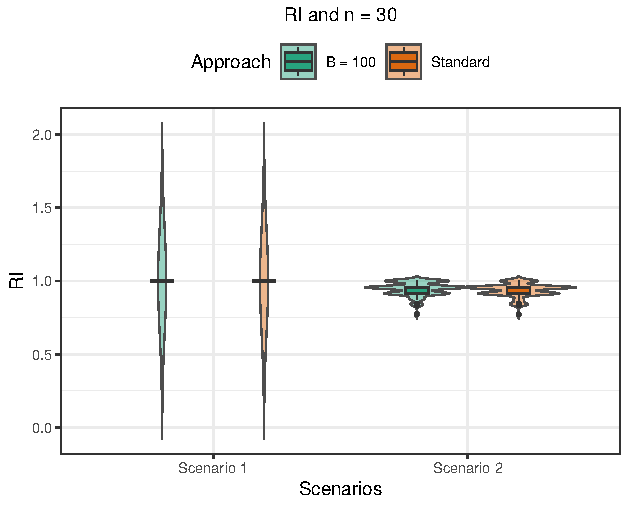
\includegraphics[width=\linewidth]{figures/pam_violin_IR_bing_k4_n30.pdf}
  \caption{RI, $n=30$.}
\end{subfigure}\hfill
\begin{subfigure}{0.46\textwidth}\centering
  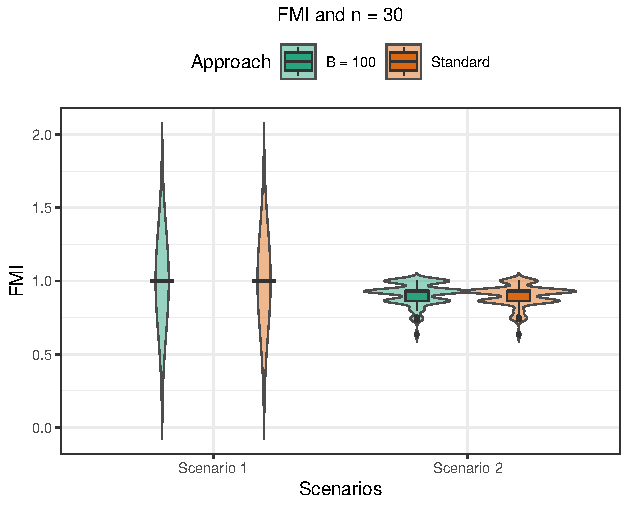
\includegraphics[width=\linewidth]{figures/pam_violin_IFM_bing_k4_n30.pdf}
  \caption{FMI, $n=30$.}
\end{subfigure}

\vspace{0.4em}

\begin{subfigure}{0.46\textwidth}\centering
  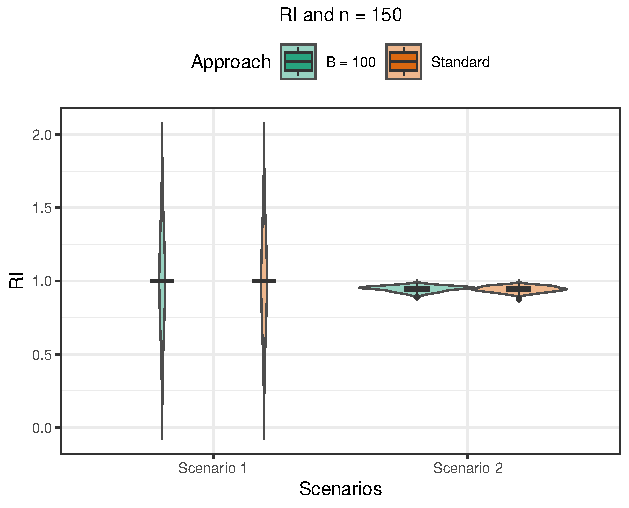
\includegraphics[width=\linewidth]{figures/pam_violin_IR_bing_k4_n150.pdf}
  \caption{RI, $n=150$.}
\end{subfigure}\hfill
\begin{subfigure}{0.46\textwidth}\centering
  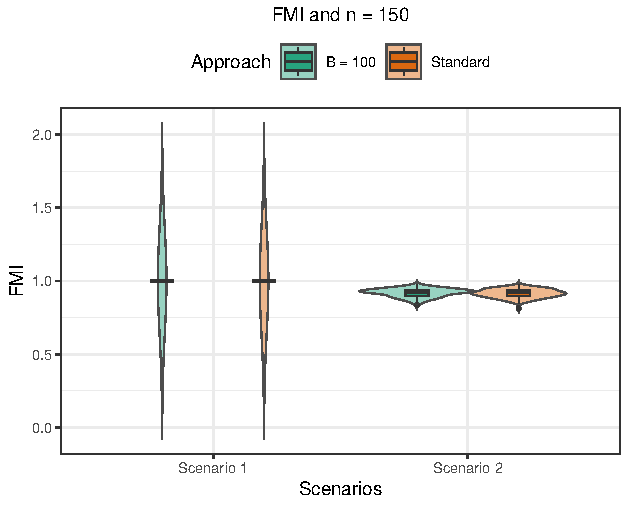
\includegraphics[width=\linewidth]{figures/pam_violin_IFM_bing_k4_n150.pdf}
  \caption{FMI, $n=150$.}
\end{subfigure}
\caption{Shape-PAM vs.\ PAM-Bagging on Bingham pre-shape data, $k=4$.}
\label{fig:viol-pam-bing-k4}
\end{figure}

\begin{figure}[h]
\centering
\begin{subfigure}{0.46\textwidth}\centering
  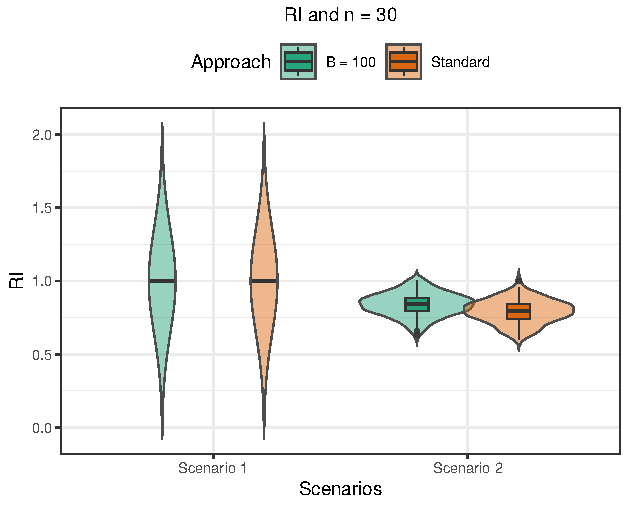
\includegraphics[width=\linewidth]{figures/pam_violin_IR_bing_k24_n30.pdf}
  \caption{RI, $n=30$.}
\end{subfigure}\hfill
\begin{subfigure}{0.46\textwidth}\centering
  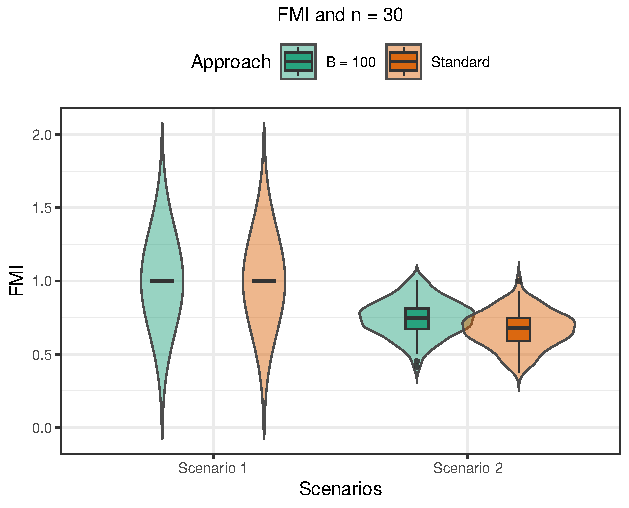
\includegraphics[width=\linewidth]{figures/pam_violin_IFM_bing_k24_n30.pdf}
  \caption{FMI, $n=30$.}
\end{subfigure}

\vspace{0.4em}

\begin{subfigure}{0.46\textwidth}\centering
  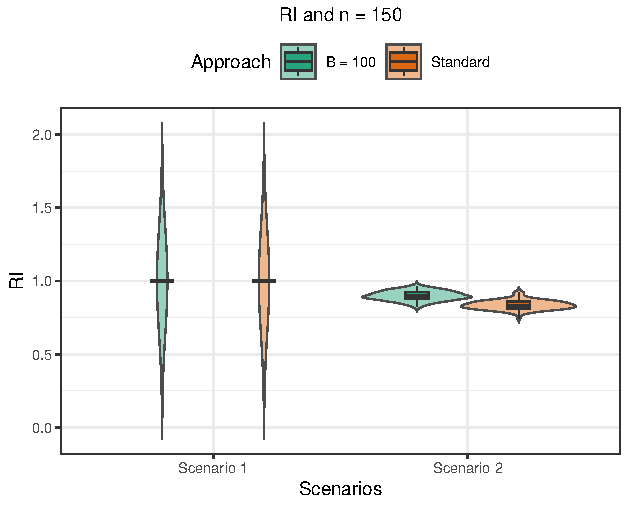
\includegraphics[width=\linewidth]{figures/pam_violin_IR_bing_k24_n150.pdf}
  \caption{RI, $n=150$.}
\end{subfigure}\hfill
\begin{subfigure}{0.46\textwidth}\centering
  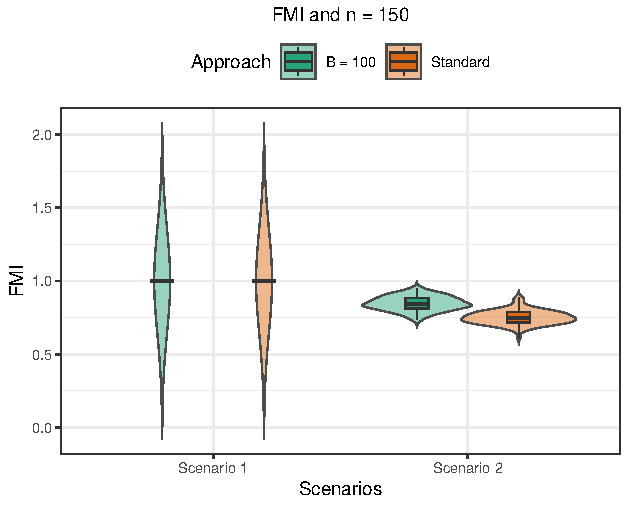
\includegraphics[width=\linewidth]{figures/pam_violin_IFM_bing_k24_n150.pdf}
  \caption{FMI, $n=150$.}
\end{subfigure}
\caption{Shape-PAM vs.\ PAM-Bagging on Bingham pre-shape data, $k=24$.}
\label{fig:viol-pam-bing-k24}
\end{figure}

\begin{figure}[h]
\centering
\begin{subfigure}{0.46\textwidth}\centering
  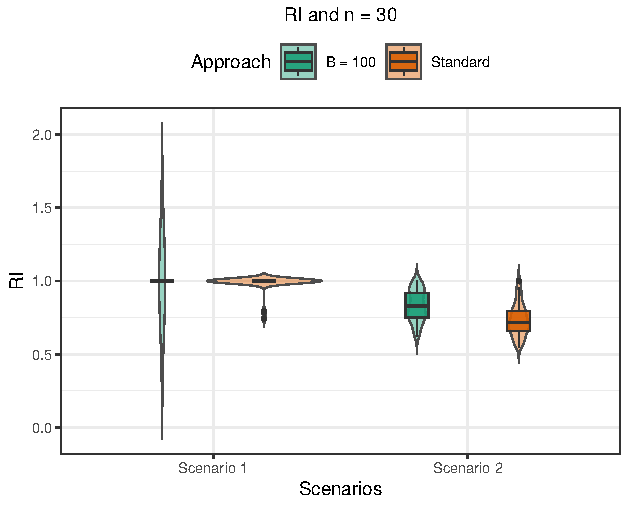
\includegraphics[width=\linewidth]{figures/rankkmed_violin_IR_bing_k4_n30.pdf}
  \caption{RI, $n=30$.}
\end{subfigure}\hfill
\begin{subfigure}{0.46\textwidth}\centering
  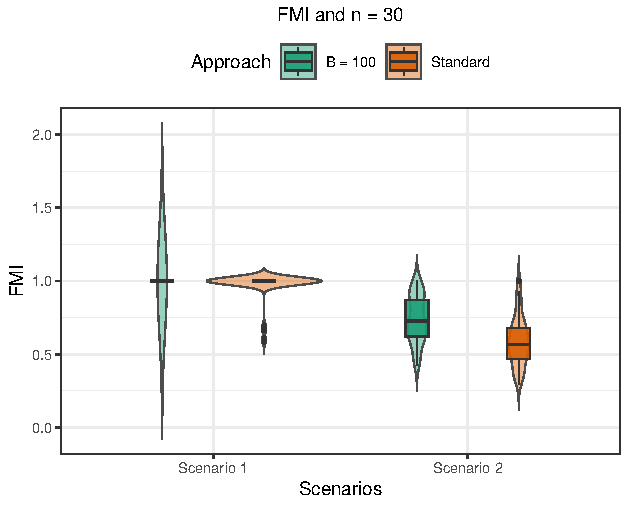
\includegraphics[width=\linewidth]{figures/rankkmed_violin_IFM_bing_k4_n30.pdf}
  \caption{FMI, $n=30$.}
\end{subfigure}

\vspace{0.4em}

\begin{subfigure}{0.46\textwidth}\centering
  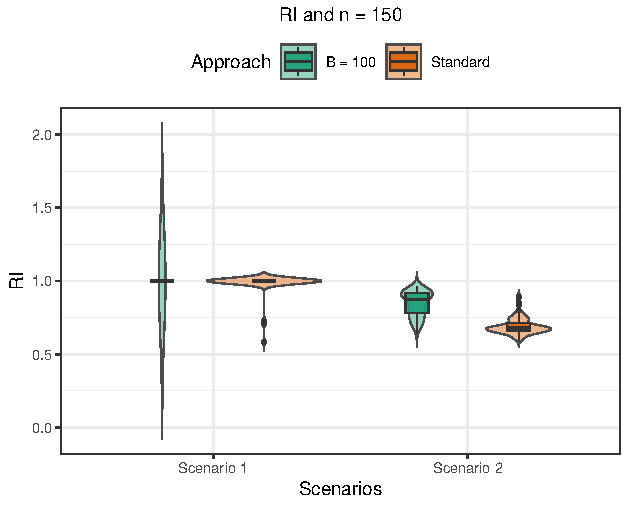
\includegraphics[width=\linewidth]{figures/rankkmed_violin_IR_bing_k4_n150.pdf}
  \caption{RI, $n=150$.}
\end{subfigure}\hfill
\begin{subfigure}{0.46\textwidth}\centering
  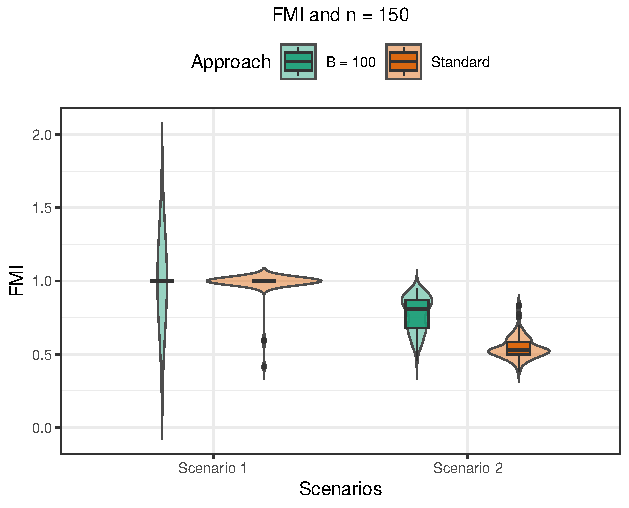
\includegraphics[width=\linewidth]{figures/rankkmed_violin_IFM_bing_k4_n150.pdf}
  \caption{FMI, $n=150$.}
\end{subfigure}
\caption{Shape-rankkmed vs.\ rankkmed-Bagging on Bingham pre-shape data,
  $k=4$.}
\label{fig:viol-rkm-bing-k4}
\end{figure}

\begin{figure}[h]
\centering
\begin{subfigure}{0.46\textwidth}\centering
  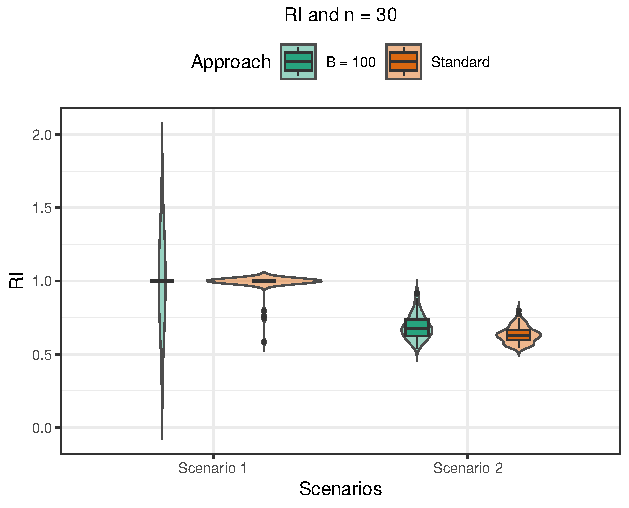
\includegraphics[width=\linewidth]{figures/rankkmed_violin_IR_bing_k24_n30.pdf}
  \caption{RI, $n=30$.}
\end{subfigure}\hfill
\begin{subfigure}{0.46\textwidth}\centering
  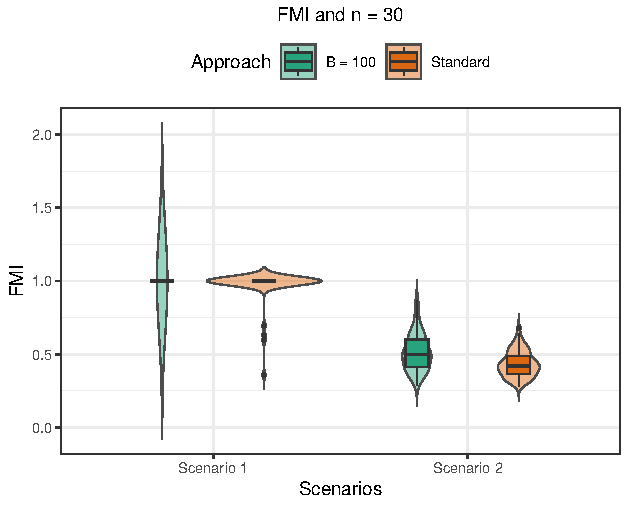
\includegraphics[width=\linewidth]{figures/rankkmed_violin_IFM_bing_k24_n30.pdf}
  \caption{FMI, $n=30$.}
\end{subfigure}

\vspace{0.4em}

\begin{subfigure}{0.46\textwidth}\centering
  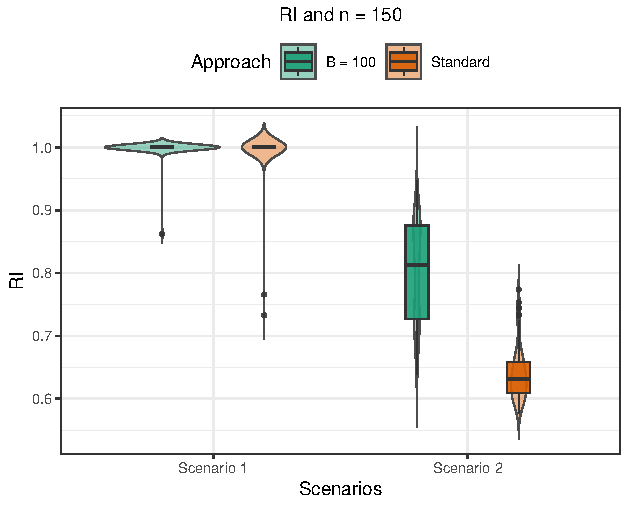
\includegraphics[width=\linewidth]{figures/rankkmed_violin_IR_bing_k24_n150.pdf}
  \caption{RI, $n=150$.}
\end{subfigure}\hfill
\begin{subfigure}{0.46\textwidth}\centering
  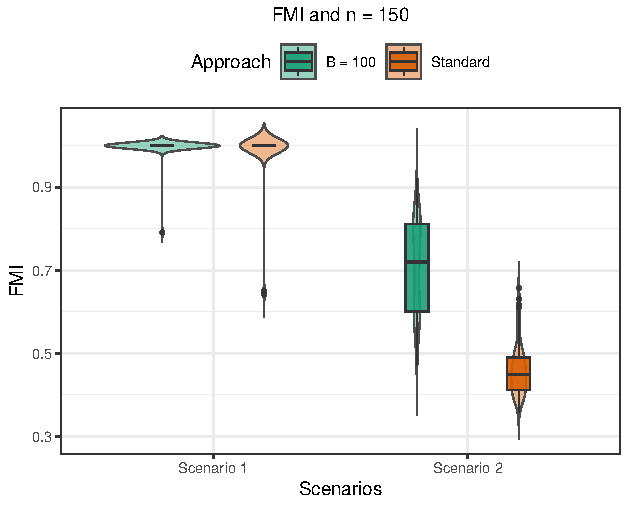
\includegraphics[width=\linewidth]{figures/rankkmed_violin_IFM_bing_k24_n150.pdf}
  \caption{FMI, $n=150$.}
\end{subfigure}
\caption{Shape-rankkmed vs.\ rankkmed-Bagging on Bingham pre-shape data,
  $k=24$.}
\label{fig:viol-rkm-bing-k24}
\end{figure}

\begin{figure}[h]
\centering
\begin{subfigure}{0.46\textwidth}\centering
  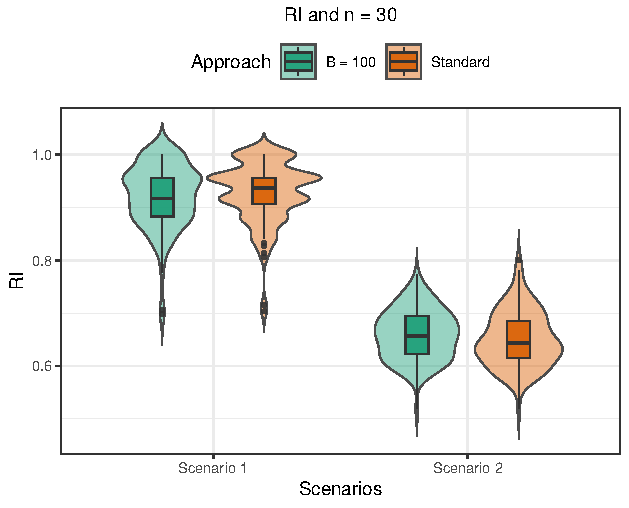
\includegraphics[width=\linewidth]{figures/pam_violin_IR_iso_k4_n30.pdf}
  \caption{RI, $n=30$.}
\end{subfigure}\hfill
\begin{subfigure}{0.46\textwidth}\centering
  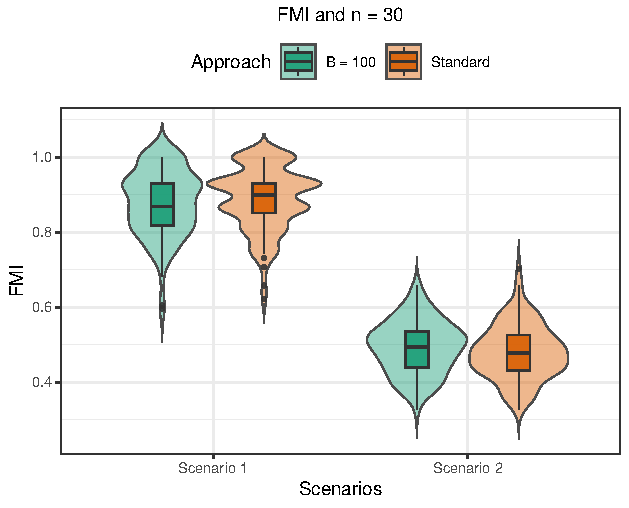
\includegraphics[width=\linewidth]{figures/pam_violin_IFM_iso_k4_n30.pdf}
  \caption{FMI, $n=30$.}
\end{subfigure}

\vspace{0.4em}

\begin{subfigure}{0.46\textwidth}\centering
  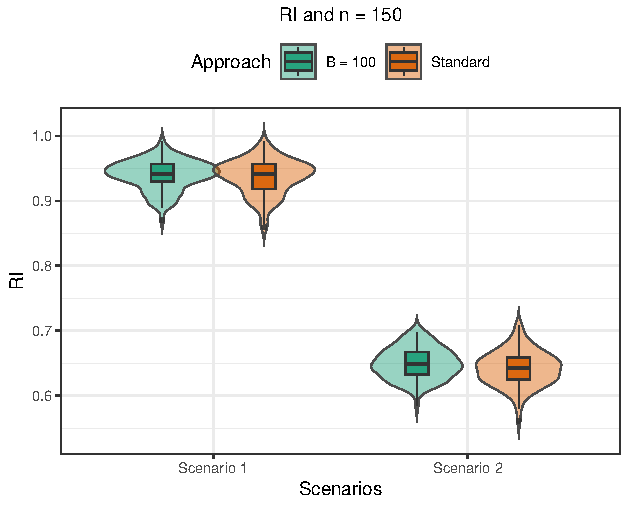
\includegraphics[width=\linewidth]{figures/pam_violin_IR_iso_k4_n150.pdf}
  \caption{RI, $n=150$.}
\end{subfigure}\hfill
\begin{subfigure}{0.46\textwidth}\centering
  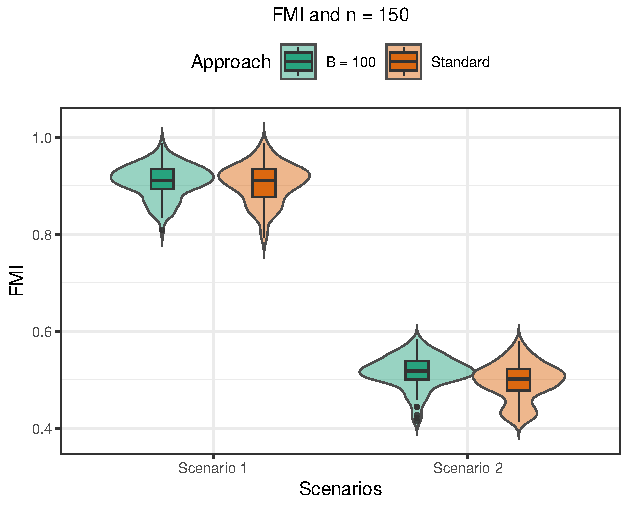
\includegraphics[width=\linewidth]{figures/pam_violin_IFM_iso_k4_n150.pdf}
  \caption{FMI, $n=150$.}
\end{subfigure}
\caption{Shape-PAM vs.\ PAM-Bagging on isotropic landmark data, $k=4$.}
\label{fig:viol-pam-iso-k4}
\end{figure}

\begin{figure}[h]
\centering
\begin{subfigure}{0.46\textwidth}\centering
  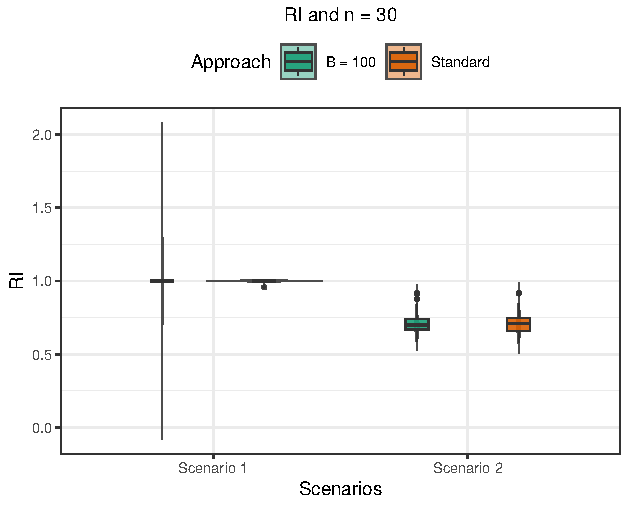
\includegraphics[width=\linewidth]{figures/pam_violin_IR_iso_k34_n30.pdf}
  \caption{RI, $n=30$.}
\end{subfigure}\hfill
\begin{subfigure}{0.46\textwidth}\centering
  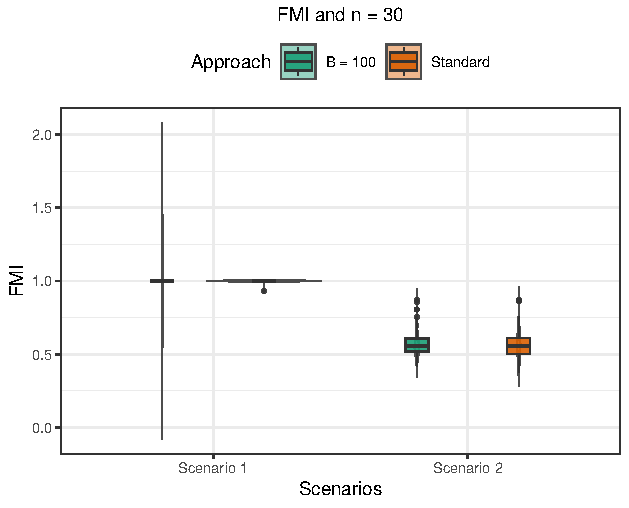
\includegraphics[width=\linewidth]{figures/pam_violin_IFM_iso_k34_n30.pdf}
  \caption{FMI, $n=30$.}
\end{subfigure}

\vspace{0.4em}

\begin{subfigure}{0.46\textwidth}\centering
  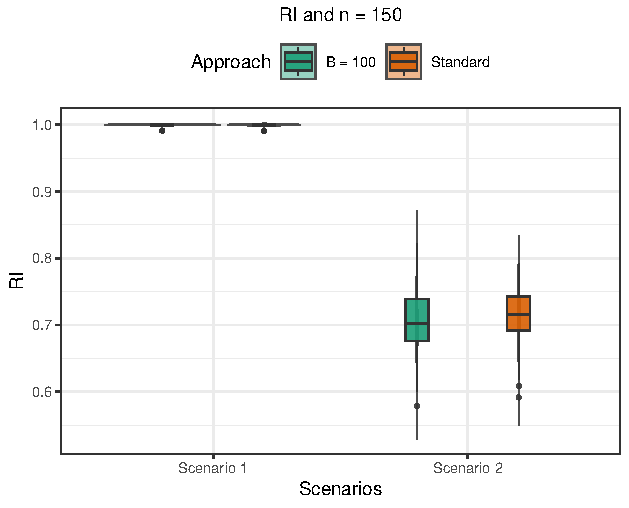
\includegraphics[width=\linewidth]{figures/pam_violin_IR_iso_k34_n150.pdf}
  \caption{RI, $n=150$.}
\end{subfigure}\hfill
\begin{subfigure}{0.46\textwidth}\centering
  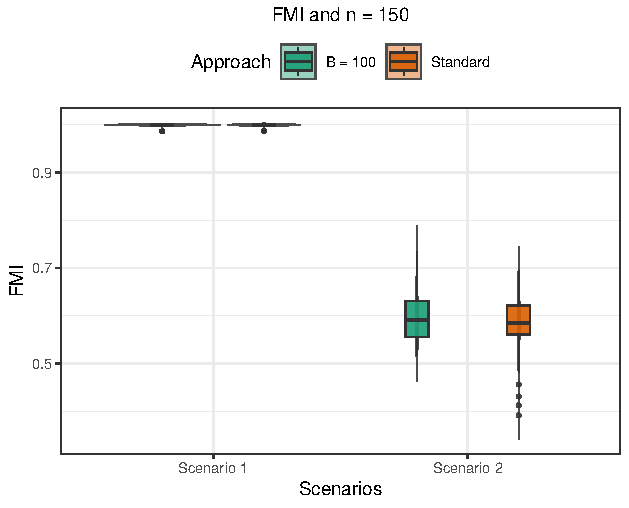
\includegraphics[width=\linewidth]{figures/pam_violin_IFM_iso_k34_n150.pdf}
  \caption{FMI, $n=150$.}
\end{subfigure}
\caption{Shape-PAM vs.\ PAM-Bagging on isotropic landmark data, $k=34$.}
\label{fig:viol-pam-iso-k34}
\end{figure}

\begin{figure}[h]
\centering
\begin{subfigure}{0.46\textwidth}\centering
  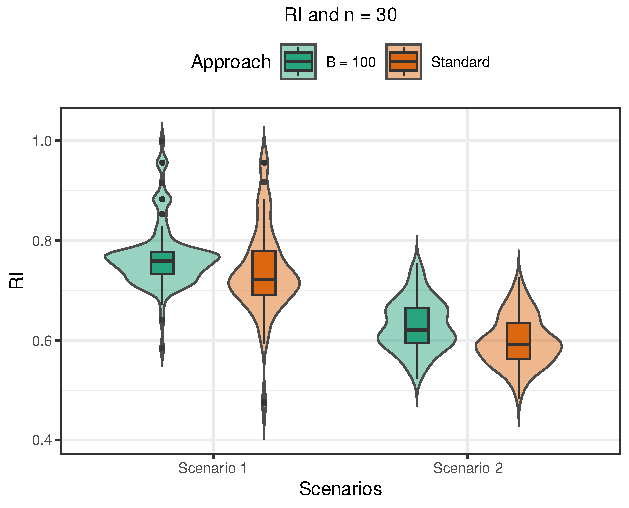
\includegraphics[width=\linewidth]{figures/rankkmed_violin_IR_iso_k4_n30.pdf}
  \caption{RI, $n=30$.}
\end{subfigure}\hfill
\begin{subfigure}{0.46\textwidth}\centering
  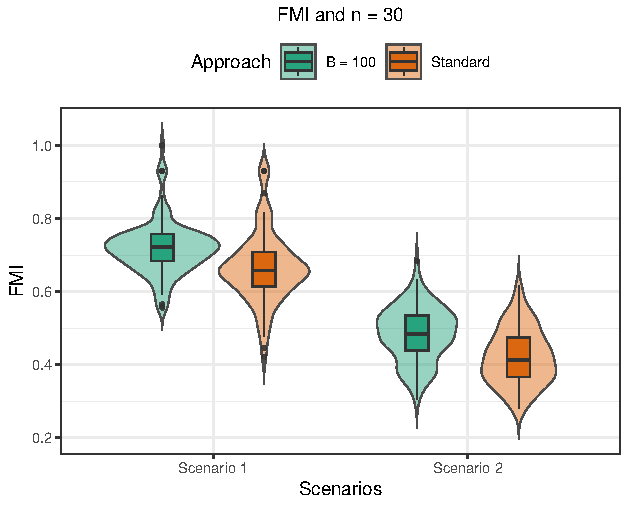
\includegraphics[width=\linewidth]{figures/rankkmed_violin_IFM_iso_k4_n30.pdf}
  \caption{FMI, $n=30$.}
\end{subfigure}

\vspace{0.4em}

\begin{subfigure}{0.46\textwidth}\centering
  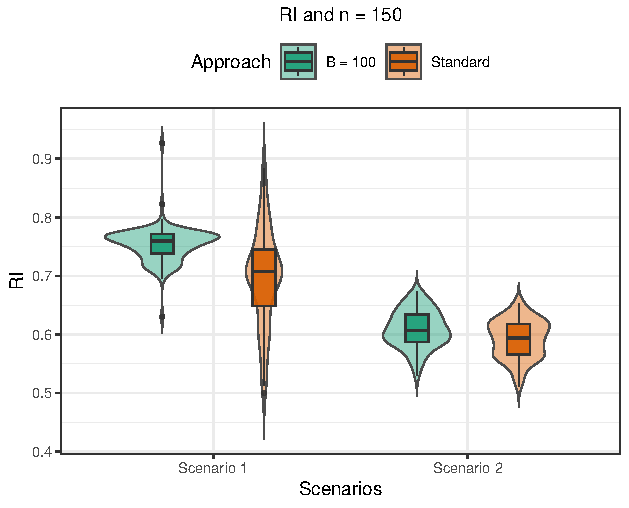
\includegraphics[width=\linewidth]{figures/rankkmed_violin_IR_iso_k4_n150.pdf}
  \caption{RI, $n=150$.}
\end{subfigure}\hfill
\begin{subfigure}{0.46\textwidth}\centering
  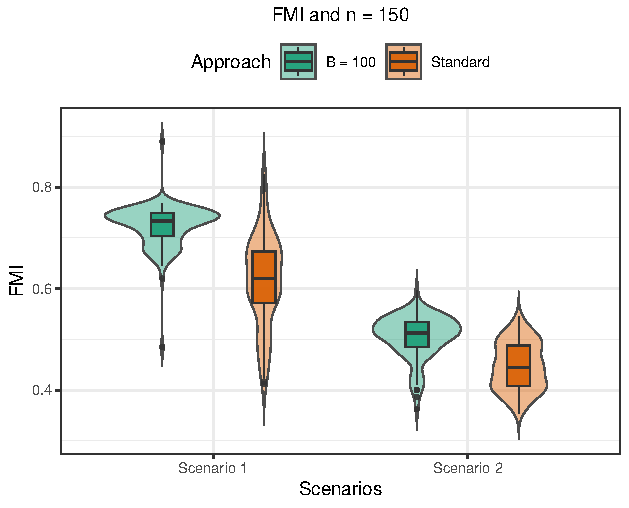
\includegraphics[width=\linewidth]{figures/rankkmed_violin_IFM_iso_k4_n150.pdf}
  \caption{FMI, $n=150$.}
\end{subfigure}
\caption{Shape-rankkmed vs.\ rankkmed-Bagging on isotropic landmark data,
  $k=4$.}
\label{fig:viol-rkm-iso-k4}
\end{figure}

\begin{figure}[h]
\centering
\begin{subfigure}{0.46\textwidth}\centering
  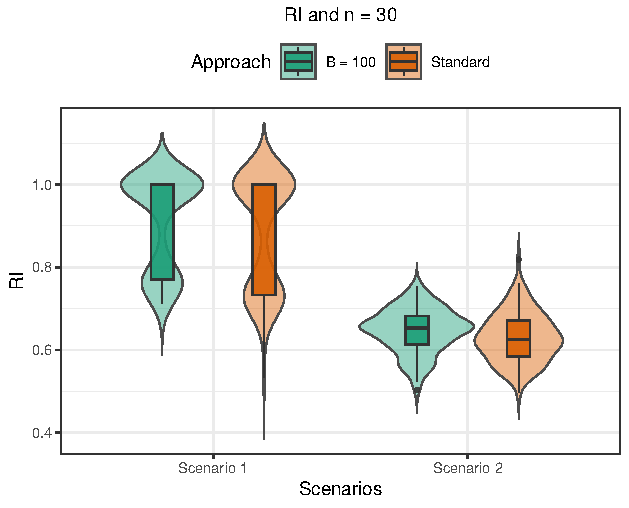
\includegraphics[width=\linewidth]{figures/rankkmed_violin_IR_iso_k34_n30.pdf}
  \caption{RI, $n=30$.}
\end{subfigure}\hfill
\begin{subfigure}{0.46\textwidth}\centering
  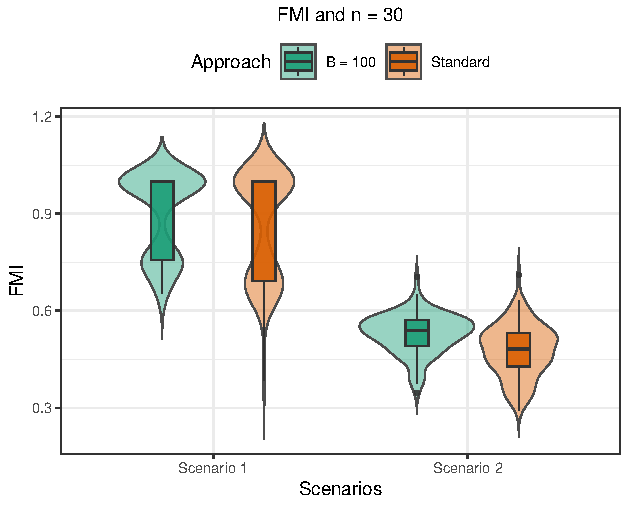
\includegraphics[width=\linewidth]{figures/rankkmed_violin_IFM_iso_k34_n30.pdf}
  \caption{FMI, $n=30$.}
\end{subfigure}

\vspace{0.4em}

\begin{subfigure}{0.46\textwidth}\centering
  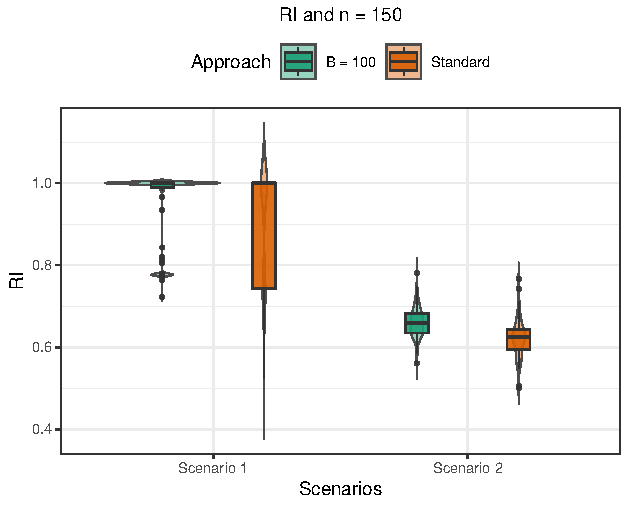
\includegraphics[width=\linewidth]{figures/rankkmed_violin_IR_iso_k34_n150.pdf}
  \caption{RI, $n=150$.}
\end{subfigure}\hfill
\begin{subfigure}{0.46\textwidth}\centering
  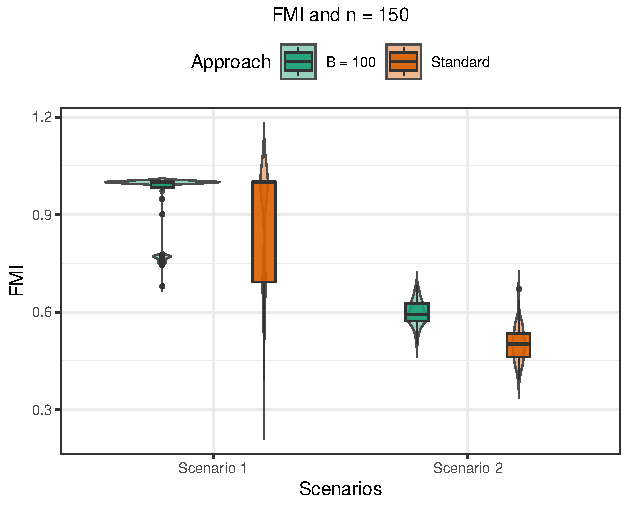
\includegraphics[width=\linewidth]{figures/rankkmed_violin_IFM_iso_k34_n150.pdf}
  \caption{FMI, $n=150$.}
\end{subfigure}
\caption{Shape-rankkmed vs.\ rankkmed-Bagging on isotropic landmark data,
  $k=34$.}
\label{fig:viol-rkm-iso-k34}
\end{figure}

\begin{figure}[h]
\centering
\begin{subfigure}{0.46\textwidth}\centering
  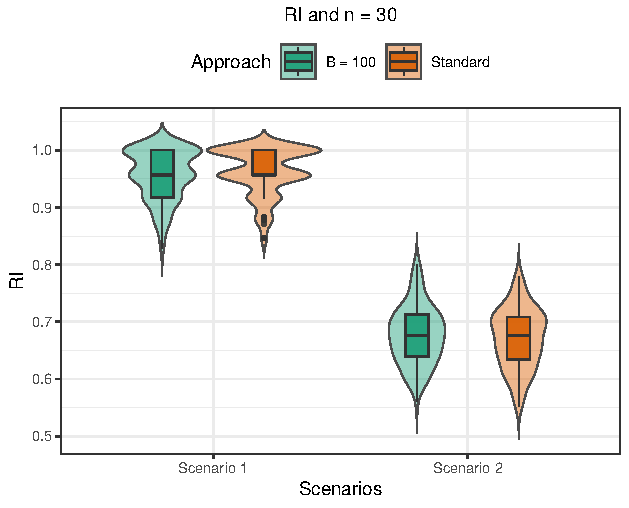
\includegraphics[width=\linewidth]{figures/pam_violin_IR_aniso_k4_n30.pdf}
  \caption{RI, $n=30$.}
\end{subfigure}\hfill
\begin{subfigure}{0.46\textwidth}\centering
  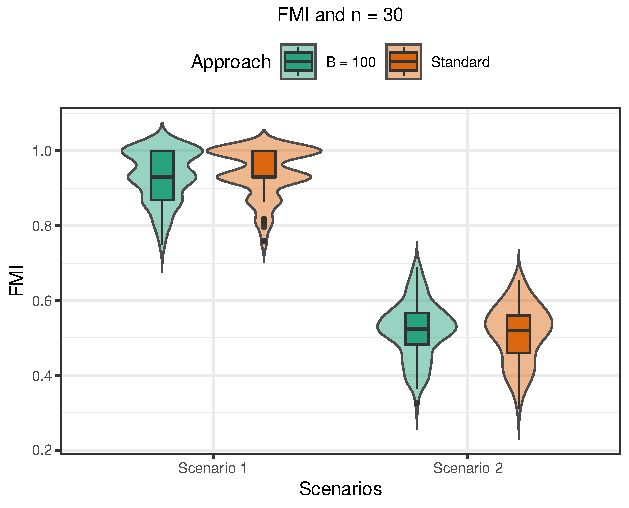
\includegraphics[width=\linewidth]{figures/pam_violin_IFM_aniso_k4_n30.pdf}
  \caption{FMI, $n=30$.}
\end{subfigure}

\vspace{0.4em}

\begin{subfigure}{0.46\textwidth}\centering
  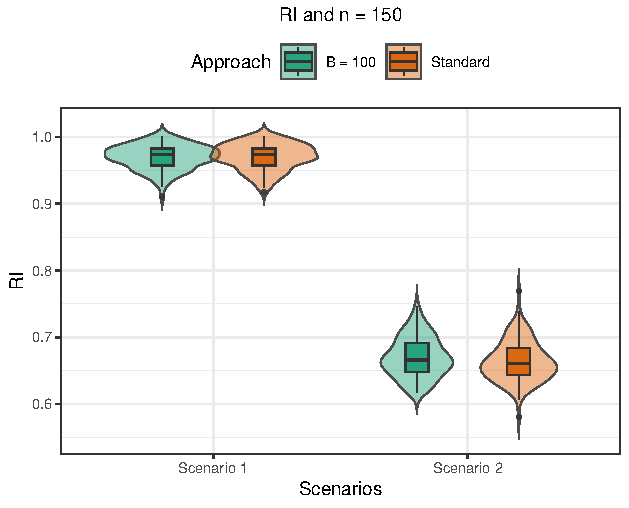
\includegraphics[width=\linewidth]{figures/pam_violin_IR_aniso_k4_n150.pdf}
  \caption{RI, $n=150$.}
\end{subfigure}\hfill
\begin{subfigure}{0.46\textwidth}\centering
  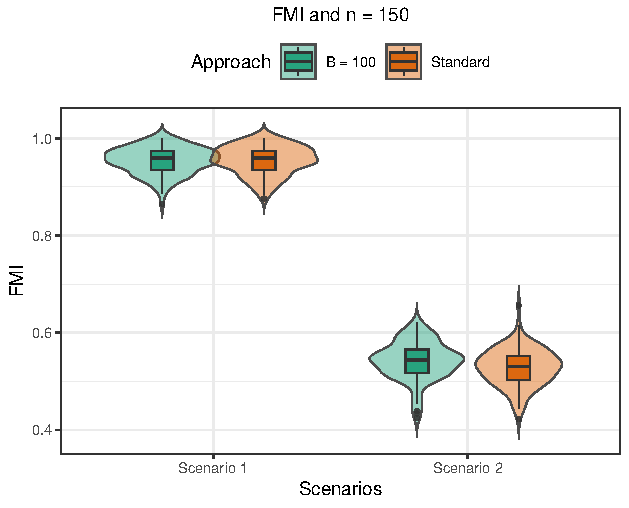
\includegraphics[width=\linewidth]{figures/pam_violin_IFM_aniso_k4_n150.pdf}
  \caption{FMI, $n=150$.}
\end{subfigure}
\caption{Shape-PAM vs.\ PAM-Bagging on anisotropic landmark data, $k=4$.}
\label{fig:viol-pam-aniso-k4}
\end{figure}

\begin{figure}[h]
\centering
\begin{subfigure}{0.46\textwidth}\centering
  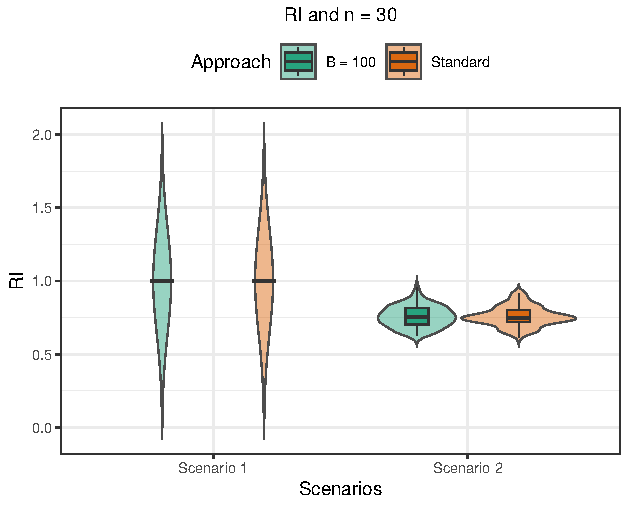
\includegraphics[width=\linewidth]{figures/pam_violin_IR_aniso_k34_n30.pdf}
  \caption{RI, $n=30$.}
\end{subfigure}\hfill
\begin{subfigure}{0.46\textwidth}\centering
  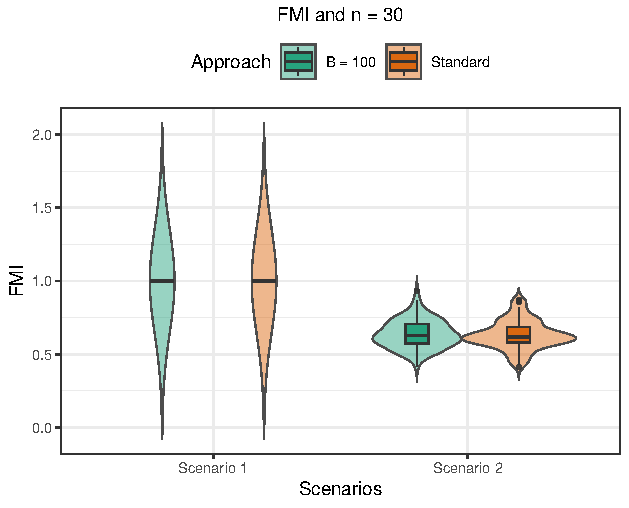
\includegraphics[width=\linewidth]{figures/pam_violin_IFM_aniso_k34_n30.pdf}
  \caption{FMI, $n=30$.}
\end{subfigure}

\vspace{0.4em}

\begin{subfigure}{0.46\textwidth}\centering
  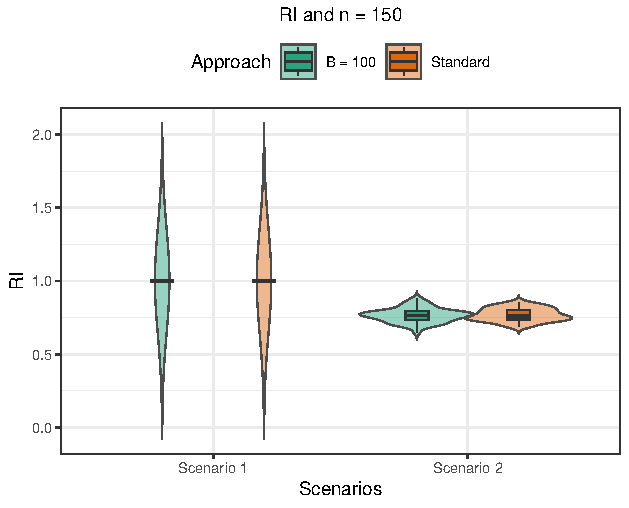
\includegraphics[width=\linewidth]{figures/pam_violin_IR_aniso_k34_n150.pdf}
  \caption{RI, $n=150$.}
\end{subfigure}\hfill
\begin{subfigure}{0.46\textwidth}\centering
  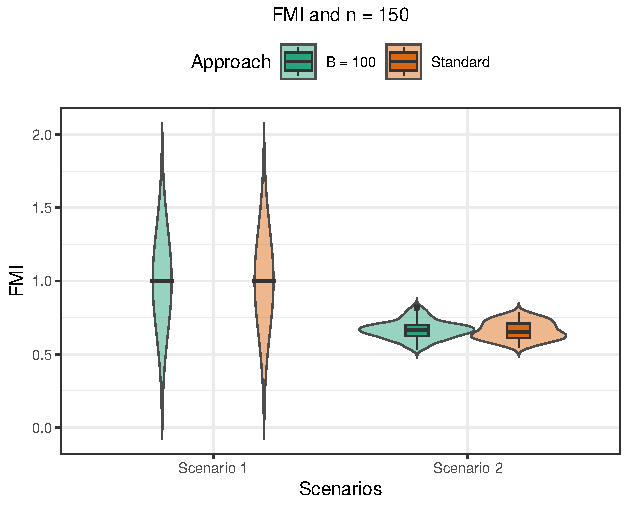
\includegraphics[width=\linewidth]{figures/pam_violin_IFM_aniso_k34_n150.pdf}
  \caption{FMI, $n=150$.}
\end{subfigure}
\caption{Shape-PAM vs.\ PAM-Bagging on anisotropic landmark data, $k=34$.}
\label{fig:viol-pam-aniso-k34}
\end{figure}

\begin{figure}[h]
\centering
\begin{subfigure}{0.46\textwidth}\centering
  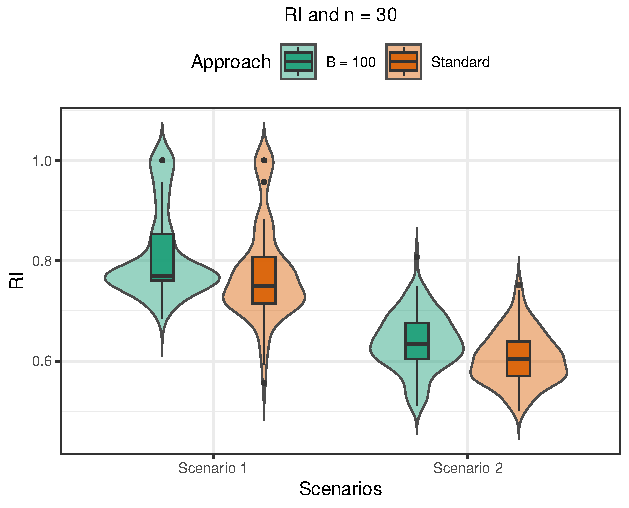
\includegraphics[width=\linewidth]{figures/rankkmed_violin_IR_aniso_k4_n30.pdf}
  \caption{RI, $n=30$.}
\end{subfigure}\hfill
\begin{subfigure}{0.46\textwidth}\centering
  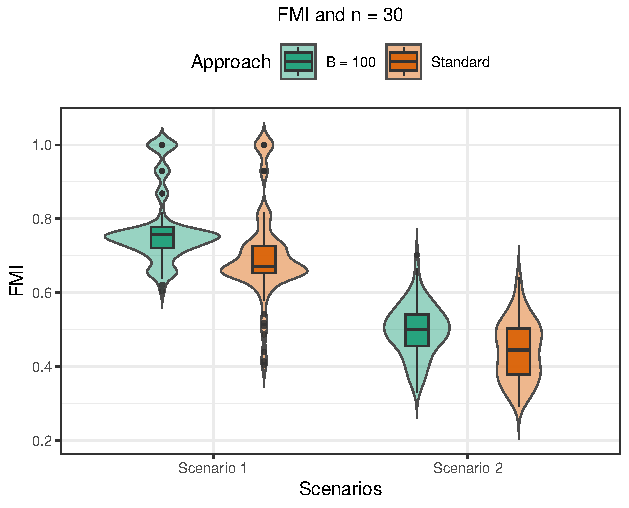
\includegraphics[width=\linewidth]{figures/rankkmed_violin_IFM_aniso_k4_n30.pdf}
  \caption{FMI, $n=30$.}
\end{subfigure}

\vspace{0.4em}

\begin{subfigure}{0.46\textwidth}\centering
  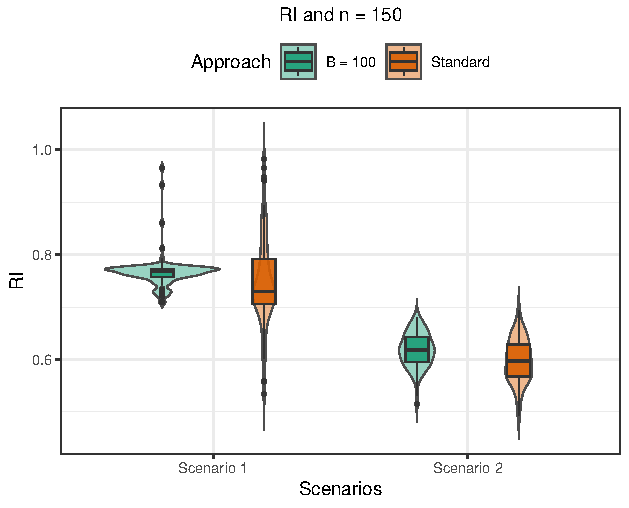
\includegraphics[width=\linewidth]{figures/rankkmed_violin_IR_aniso_k4_n150.pdf}
  \caption{RI, $n=150$.}
\end{subfigure}\hfill
\begin{subfigure}{0.46\textwidth}\centering
  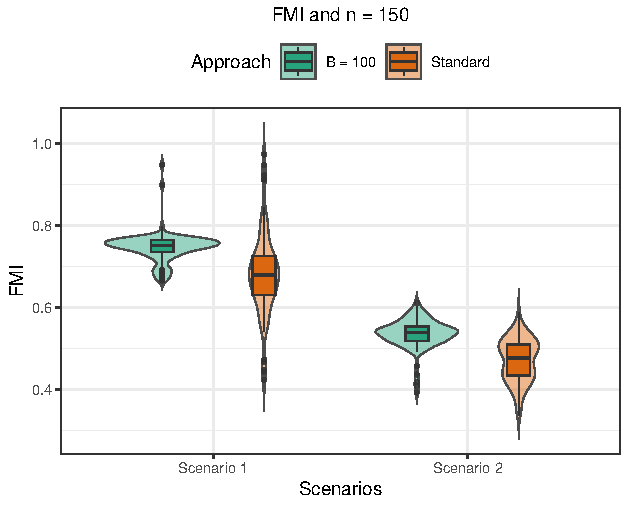
\includegraphics[width=\linewidth]{figures/rankkmed_violin_IFM_aniso_k4_n150.pdf}
  \caption{FMI, $n=150$.}
\end{subfigure}
\caption{Shape-rankkmed vs.\ rankkmed-Bagging on anisotropic landmark
  data, $k=4$.}
\label{fig:viol-rkm-aniso-k4}
\end{figure}

\begin{figure}[h]
\centering
\begin{subfigure}{0.46\textwidth}\centering
  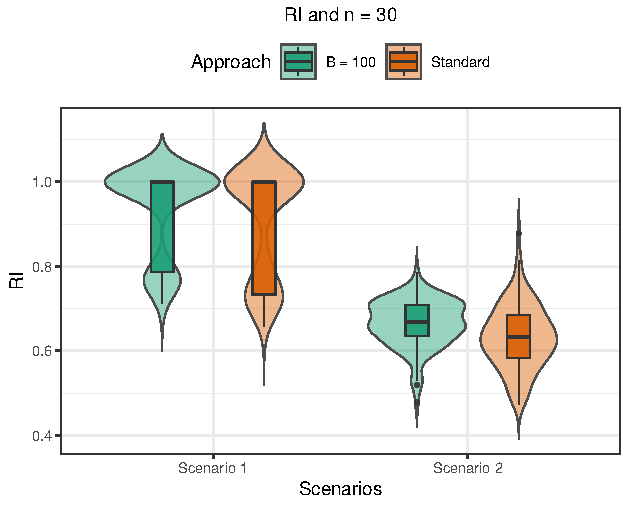
\includegraphics[width=\linewidth]{figures/rankkmed_violin_IR_aniso_k34_n30.pdf}
  \caption{RI, $n=30$.}
\end{subfigure}\hfill
\begin{subfigure}{0.46\textwidth}\centering
  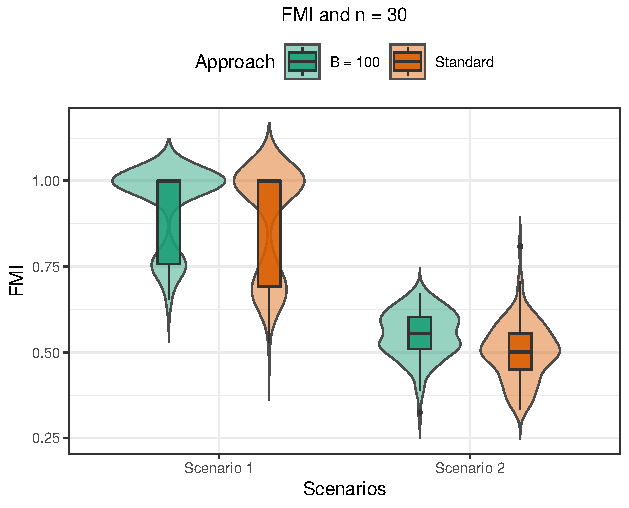
\includegraphics[width=\linewidth]{figures/rankkmed_violin_IFM_aniso_k34_n30.pdf}
  \caption{FMI, $n=30$.}
\end{subfigure}

\vspace{0.4em}

\begin{subfigure}{0.46\textwidth}\centering
  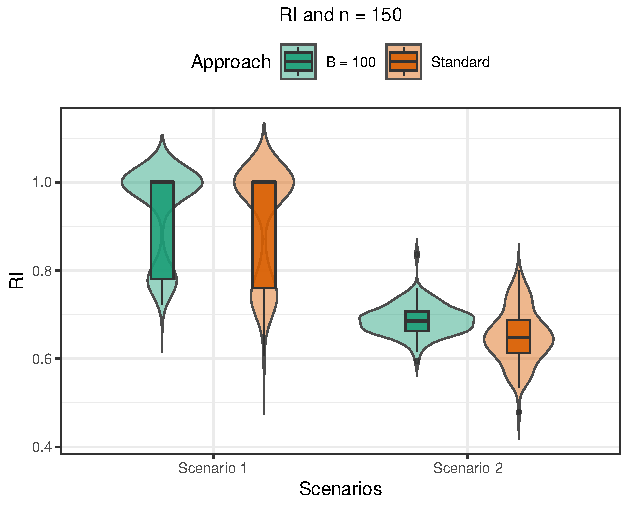
\includegraphics[width=\linewidth]{figures/rankkmed_violin_IR_aniso_k34_n150.pdf}
  \caption{RI, $n=150$.}
\end{subfigure}\hfill
\begin{subfigure}{0.46\textwidth}\centering
  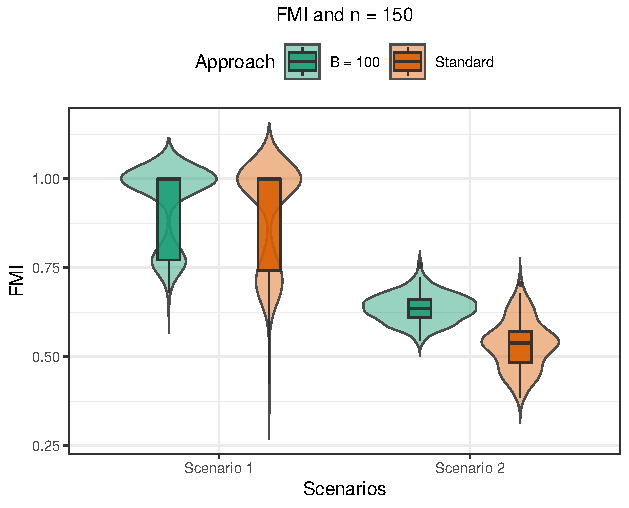
\includegraphics[width=\linewidth]{figures/rankkmed_violin_IFM_aniso_k34_n150.pdf}
  \caption{FMI, $n=150$.}
\end{subfigure}
\caption{Shape-rankkmed vs.\ rankkmed-Bagging on anisotropic landmark
  data, $k=34$.}
\label{fig:viol-rkm-aniso-k34}
\end{figure}

\clearpage


% =====================================================================
\section{Wall-clock time tables}
\label{sec:time}
% =====================================================================

For each regime and base clusterer we report the mean execution time, in
minutes, of the bagging procedure with $B=100$, both with and without
parallelization across three logical processors. The reported gains
support the claim in Section~5 of the main paper that the parallel
speedup is between $32\%$ and $77\%$ across all configurations.

\begin{table}[h]
\centering
\caption{Bagging-PAM execution time, Bingham pre-shape regime (minutes).}
\label{tab:time-pam-bing}
\small
\begin{tabular}{cc cc cc}
\toprule
& & \multicolumn{2}{c}{$k=4$} & \multicolumn{2}{c}{$k=24$} \\
\cmidrule(lr){3-4}\cmidrule(lr){5-6}
$n$ & Conc.\ & No par.\ & Par.\ & No par.\ & Par.\ \\
\midrule
$30$  & 1 & $0.152$ & $0.077$ & $0.234$ & $0.177$ \\
      & 2 & $0.121$ & $0.092$ & $0.205$ & $0.157$ \\
$150$ & 1 & $7.009$ & $3.505$ & $2.516$ & $1.258$ \\
      & 2 & $2.105$ & $1.403$ & $4.787$ & $2.992$ \\
\bottomrule
\end{tabular}
\end{table}

\begin{table}[h]
\centering
\caption{Bagging-rankkmed execution time, Bingham pre-shape regime
  (minutes).}
\label{tab:time-rkm-bing}
\small
\begin{tabular}{cc cc cc}
\toprule
& & \multicolumn{2}{c}{$k=4$} & \multicolumn{2}{c}{$k=24$} \\
\cmidrule(lr){3-4}\cmidrule(lr){5-6}
$n$ & Conc.\ & No par.\ & Par.\ & No par.\ & Par.\ \\
\midrule
$30$  & 1 & $0.249$ & $0.142$ & $0.563$ & $0.322$ \\
      & 2 & $0.381$ & $0.272$ & $0.403$ & $0.268$ \\
$150$ & 1 & $3.213$ & $1.691$ & $4.478$ & $2.634$ \\
      & 2 & $3.371$ & $1.822$ & $5.302$ & $3.314$ \\
\bottomrule
\end{tabular}
\end{table}

\begin{table}[h]
\centering
\caption{Bagging-PAM execution time, isotropic landmark regime
  (minutes).}
\label{tab:time-pam-iso}
\small
\begin{tabular}{cc cc cc}
\toprule
& & \multicolumn{2}{c}{$k=4$} & \multicolumn{2}{c}{$k=34$} \\
\cmidrule(lr){3-4}\cmidrule(lr){5-6}
$n$ & Cen.\ & No par.\ & Par.\ & No par.\ & Par.\ \\
\midrule
$30$  & 1 & $0.127$ & $0.144$ & $0.342$ & $0.252$ \\
      & 2 & $0.136$ & $0.142$ & $0.491$ & $0.322$ \\
$150$ & 1 & $2.358$ & $1.220$ & $7.727$ & $4.576$ \\
      & 2 & $2.467$ & $1.281$ & $8.172$ & $4.695$ \\
\bottomrule
\end{tabular}
\end{table}

\begin{table}[h]
\centering
\caption{Bagging-rankkmed execution time, isotropic landmark regime
  (minutes).}
\label{tab:time-rkm-iso}
\small
\begin{tabular}{cc cc cc}
\toprule
& & \multicolumn{2}{c}{$k=4$} & \multicolumn{2}{c}{$k=34$} \\
\cmidrule(lr){3-4}\cmidrule(lr){5-6}
$n$ & Cen.\ & No par.\ & Par.\ & No par.\ & Par.\ \\
\midrule
$30$  & 1 & $0.344$ & $0.223$ & $0.677$ & $0.423$ \\
      & 2 & $0.353$ & $0.224$ & $0.592$ & $0.339$ \\
$150$ & 1 & $2.605$ & $1.400$ & $7.578$ & $4.425$ \\
      & 2 & $3.676$ & $1.923$ & $7.329$ & $4.077$ \\
\bottomrule
\end{tabular}
\end{table}

\begin{table}[h]
\centering
\caption{Bagging-PAM execution time, anisotropic landmark regime
  (minutes).}
\label{tab:time-pam-aniso}
\small
\begin{tabular}{cc cc cc}
\toprule
& & \multicolumn{2}{c}{$k=4$} & \multicolumn{2}{c}{$k=34$} \\
\cmidrule(lr){3-4}\cmidrule(lr){5-6}
$n$ & Cen.\ & No par.\ & Par.\ & No par.\ & Par.\ \\
\midrule
$30$  & 1 & $0.109$ & $0.134$ & $0.360$ & $0.237$ \\
      & 2 & $0.104$ & $0.127$ & $0.356$ & $0.242$ \\
$75$  & 1 & $0.636$ & $0.357$ & $1.885$ & $1.145$ \\
      & 2 & $0.682$ & $0.388$ & $1.904$ & $1.153$ \\
$150$ & 1 & $2.369$ & $1.281$ & $7.475$ & $4.445$ \\
      & 2 & $2.384$ & $1.246$ & $7.560$ & $4.449$ \\
\bottomrule
\end{tabular}
\end{table}

\begin{table}[h]
\centering
\caption{Bagging-rankkmed execution time, anisotropic landmark regime
  (minutes).}
\label{tab:time-rkm-aniso}
\small
\begin{tabular}{cc cc cc}
\toprule
& & \multicolumn{2}{c}{$k=4$} & \multicolumn{2}{c}{$k=34$} \\
\cmidrule(lr){3-4}\cmidrule(lr){5-6}
$n$ & Cen.\ & No par.\ & Par.\ & No par.\ & Par.\ \\
\midrule
$30$  & 1 & $0.362$ & $0.227$ & $0.622$ & $0.384$ \\
      & 2 & $0.348$ & $0.223$ & $0.635$ & $0.378$ \\
$75$  & 1 & $0.895$ & $0.494$ & $2.065$ & $1.259$ \\
      & 2 & $0.850$ & $0.464$ & $2.052$ & $1.186$ \\
$150$ & 1 & $2.768$ & $1.505$ & $7.322$ & $4.176$ \\
      & 2 & $2.665$ & $1.455$ & $7.140$ & $4.049$ \\
\bottomrule
\end{tabular}
\end{table}

\clearpage


% =====================================================================
\section{Real-world biplots and timing}
\label{sec:real-extra}
% =====================================================================

\begin{figure}[h]
\centering
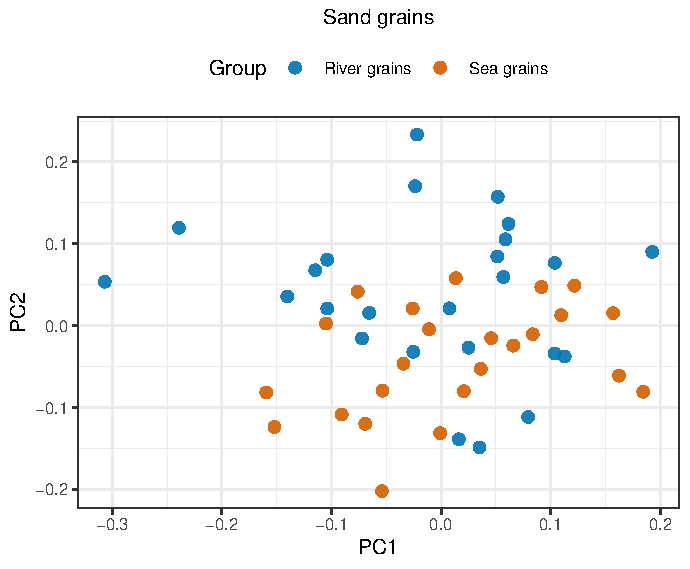
\includegraphics[width=0.65\textwidth]{figures/sand_pca.pdf}
\caption{Biplot of the sand-grains dataset, first two Riemannian principal
  components.}
\label{fig:sand-pca}
\end{figure}

\begin{figure}[h]
\centering
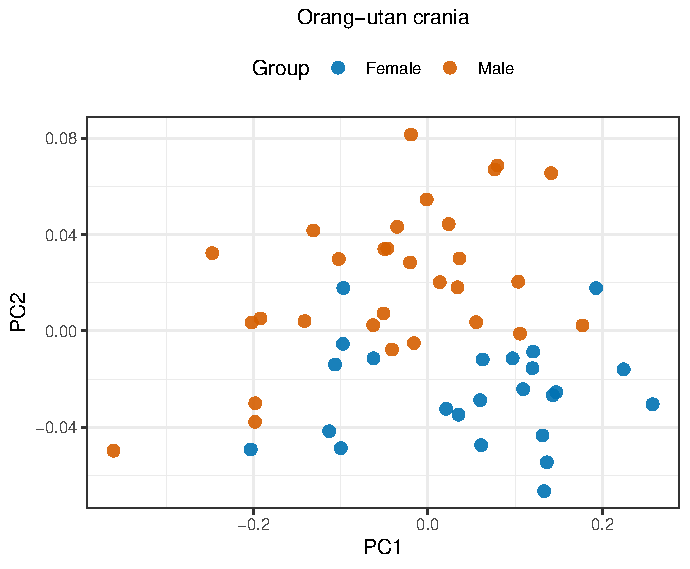
\includegraphics[width=0.65\textwidth]{figures/orang_pca.pdf}
\caption{Biplot of the orang-utan crania dataset, first two Riemannian
  principal components.}
\label{fig:orang-pca}
\end{figure}

\begin{table}[h]
\centering
\caption{Execution time (minutes) of the bagging procedure on the two
  real datasets, with and without parallelization.}
\label{tab:time-real}
\small
\begin{tabular}{lcc cc}
\toprule
& \multicolumn{2}{c}{Sand grains} & \multicolumn{2}{c}{Orang-utan crania} \\
\cmidrule(lr){2-3}\cmidrule(lr){4-5}
Algorithm & No par.\ & Par.\ & No par.\ & Par.\ \\
\midrule
PAM       & $0.533$ & $0.272$ & $0.533$ & $0.272$ \\
rankkmed  & $1.202$ & $0.269$ & $1.202$ & $0.269$ \\
\bottomrule
\end{tabular}
\end{table}

\clearpage


% =====================================================================
\section{Sensitivity to the choice of shape-space distance}
\label{sec:dF-sensitivity}

The main paper adopts the intrinsic Riemannian distance $\rho$. To check that
the conclusions are not an artifact of that choice, we re-ran the three hardest
scenarios --- the overlapping setting with the larger landmark count and
$n=150$, in each of the three data-generating regimes --- using the full
Procrustes distance $d_F$ instead, with the same $100$ Monte~Carlo replications
and the same $B=100$ bootstrap replicates. Table~\ref{tab:dF-vs-rho} places the
two sets of results side by side.

The column headed \emph{same conclusion?} answers one question: would a reader
who had run the entire study with $d_F$ instead of $\rho$ have drawn the same
inference about bagging in that scenario --- that is, does the bagged variant
move the median FMI in the same direction, and does the paired Wilcoxon test
fall on the same side of $\alpha = 0.05$? It is not a claim of numerical
agreement between the two distances, which would be too strong a demand; it
records whether the substantive conclusion survives the substitution.

Five of the six comparisons agree. The exception is Shape-PAM on the isotropic
regime, where the test is significant under $d_F$ ($p<0.001$) but sits just
above the threshold under $\rho$ ($p=0.051$). The direction of the effect is the
same under both distances, bagging raising the median FMI, so the disagreement
concerns where a borderline $p$-value falls relative to a conventional cutoff,
not whether bagging helps. We report it rather than suppress it: it is a
reminder that the isotropic Shape-PAM result is the weakest in the study, which
is also visible in the main paper, where that same $p$-value of $0.051$ is
printed without being marked as significant.

\begin{table}[h]
\centering
\caption{Median FMI (base $\to$ bagged) and one-sided paired Wilcoxon $p$-values
  under the Riemannian distance $\rho$ and under the full Procrustes distance
  $d_F$, in the hardest scenario of each regime ($n=150$, overlapping groups).
  Both rest on $100$ Monte~Carlo replications with $B=100$. The last column
  records whether the substantive conclusion about bagging is unchanged by the
  substitution: same direction of the median shift, and same side of
  $\alpha=0.05$.}
\label{tab:dF-vs-rho}
\small
\begin{tabular}{llccccc}
\toprule
& & \multicolumn{2}{c}{\textbf{Riemannian $\rho$}}
  & \multicolumn{2}{c}{\textbf{Full Procrustes $d_F$}} & \\
\cmidrule(lr){3-4}\cmidrule(lr){5-6}
Regime & Algorithm & FMI & $p$ & FMI & $p$ & Same conclusion? \\
\midrule
\multirow{2}{*}{Bingham, $k=24$}
 & Shape-PAM      & $0.747\to0.842$ & $<\!0.001$ & $0.747\to0.850$ & $<\!0.001$ & yes \\
 & Shape-rankkmed & $0.449\to0.721$ & $<\!0.001$ & $0.456\to0.716$ & $<\!0.001$ & yes \\
\midrule
\multirow{2}{*}{Isotropic, $k=34$}
 & Shape-PAM      & $0.585\to0.591$ & $0.051$    & $0.489\to0.578$ & $<\!0.001$ & \textbf{no} \\
 & Shape-rankkmed & $0.502\to0.593$ & $<\!0.001$ & $0.500\to0.598$ & $<\!0.001$ & yes \\
\midrule
\multirow{2}{*}{Anisotropic, $k=34$}
 & Shape-PAM      & $0.651\to0.664$ & $0.062$    & $0.618\to0.628$ & $0.098$    & yes \\
 & Shape-rankkmed & $0.539\to0.636$ & $<\!0.001$ & $0.539\to0.634$ & $<\!0.001$ & yes \\
\bottomrule
\end{tabular}
\end{table}


\bibliography{referencias}

\end{document}
